% Início.
\documentclass{iiufrgs}

\usepackage[utf8]{inputenc}
\usepackage[T1]{fontenc}
\usepackage{color}
\usepackage{graphicx}
\usepackage{amsmath}
\usepackage{listings}
\usepackage{hyperref}

\usepackage{setspace}
\onehalfspacing

% Trechos de código.
\def\lstlistlistingname{Lista de Trechos de Código}
\def\lstlistingname{Trecho de Código}
\lstset{
    inputencoding={utf8},
    extendedchars=false,
    basicstyle=\scriptsize\color{black}\ttfamily,
    numbers=left,
    numberstyle=\scriptsize\ttfamily,
    stepnumber=1,
    numbersep=10pt,
    tabsize=4,
    frame=single,
    keywordstyle=\color{black}\textbf,
    keywordstyle=[1]\color{black}\textbf,
    keywordstyle=[2]\color{black}\textbf,
    keywordstyle=[3]\color{black}\textbf,
    keywordstyle=[4]\color{black}\textbf,
    stringstyle=\color{black}\ttfamily,
    showspaces=false,
    showtabs=false,
    xleftmargin=17pt,
    framextopmargin=4pt,
    framexleftmargin=17pt,
    framexrightmargin=5pt,
    framexbottommargin=4pt,
    showstringspaces=false
}

% Dados.
\title{A Teoria do Perigo Aplicada à Detecção de Fraude}
\author{Guimarães}{Bruno Barcarol}
\advisor{Webber}{Carine Geltrudes}
\course{\cgcc}
\location{Caxias do Sul}{}

% Documento.
\begin{document}

% Folha de rosto.
\maketitle

% Sumário.
\tableofcontents

% Lista de figuras.
\listoffigures

% Conteúdo.
\chapter{Introdução}

O crescente avanço na tecnologia de armazenamento de dados, principalmente em termos de velocidade e tamanho, permite a criação de bancos de dados complexos e detalhados. Com isso, o desenvolvimento de programas de computador que há anos atrás seriam computacionalmente inviáveis torna-se possível. Uma área fortemente influenciada por esse fator é a mineração de dados.

Definida como ``análise de bases (geralmente extensas) de dados previamente coletados para estabelecer relações e apresentar a informação de forma mais clara e útil ao proprietário dos dados'' \cite[p. 1]{Hand2001}\footnote{``Data mining is the analysis of (often large) observational data sets to find unsuspected relationships and to summarize the data in novel ways that are both understandable and useful to the data owner.''.}, a mineração de dados é associada à ideia do aproveitamento de grandes bases de dados para auxiliar o profissional em alguma tarefa, através da apresentação de padrões e relações que seriam difíceis ou impossíveis de serem encontrados pelo observador humano. As atividades envolvidas na mineração de dados são:

\begin{itemize}
\item Determinar como os dados a serem usados serão representados. As estruturas do problema devem ser codificadas para que possam ser utilizadas por algoritmos computacionais. Formas comuns de representação são cadeias de bits, números inteiros, números reais e valores categóricos.
\item Decidir a função de aptidão. Essa função é utilizada para quantificar a adequação de um modelo a um conjunto de dados, permitindo definir se um modelo é "melhor" que outro, ou seja, representa mais precisamente os elementos daquele conjunto.
\item Escolher um processo algorítmico para otimizar a função de comparação. Através de um algoritmo específico, modelos diferentes (ou parâmetros diferentes para um mesmo tipo de modelo) são criados e testados utilizando a função de aptidão. Esse processo é repetido até que a condição de término seja encontrada, geralmente após um determinado limite da função de aptidão ou um determinado número de iterações.
\item Administrar o acesso aos dados de forma eficiente durante a execução dos algoritmos. Grandes \emph{datasets} geralmente excedem o tamanho dos dispositivos de armazenamento primário atuais. Dispositivos de armazenamento secundário ou terciário são utlizados, tornando o acesso a esses dados ineficiente. Um algoritmo corre o risco de tornar-se computacionalmente inviável caso o programador não considere esse fato.
\end{itemize}

Os exemplos da sua utilização são inúmeros, estendendo-se virtualmente a qualquer atividade, de empresas comerciais à medicina e engenharia. A coleta e armazenamento de informações cresce constantemente, tornando a análise desses dados impossível sem o uso de uma ferramenta automatizada. A mineração extrai padrões ou modelos dessas fontes de informação, que seriam difíceis ou impossíveis de serem visualizadas apenas observando-se os dados. Isso tem motivado o desenvolvimento de algoritmos capazes de identificar padrões com mais detalhamento e significado.

Como área interdisciplinar, a mineração atrai estudiosos de diversas áreas da computação como, em especial, a Inteligência Artificial. A combinação de técnicas tradicionais de mineração com os algoritmos da Inteligência Artificial estende em muito o seu poder de análise. Tomando a definição básica de Luger \cite[p. 1]{Luger2009}:

\begin{quote}
``Inteligência Artificial (IA) pode ser definida como a área da ciência da computação que se dedica a automação de comportamento inteligente.''\footnote{``Artificial intelligence (AI) may be defined as the branch of computer science that is concerned with the automation of inteligent behaviour.''.}
\end{quote}

Analisar informações, raciocinar e tirar conclusões são também objeto de estudo da Inteligência Artificial. Redes neurais e bayesianas, clustering e lógica nebulosa (\emph{fuzzy}) são alguns dos métodos mais aplicados nessas situações. De fato, as grandes bases de dados que geralmente são objeto de atuação da mineração constituem excelente campo de testes para os algoritmos da IA. 

Uma área que têm recebido crescente atenção de estudos de mineração de dados e Inteligência Artificial é a de segurança da informação. O desenvolvimento de ferramentas de mineração é visto como um forte candidato à solução desses problemas, já que elas são capazes de extrair modelos e comportamentos da base de dados que dificilmente seriam percebidos por um observador humano. O ganho que um profissional tem ao utilizar uma ferramenta dessa natureza é enorme: a tarefa de análise de bases de dados extensas é passada dele para o computador. O reconhecimento de padrões e capacidade de investigação de grandes bases de dados são os maiores desafios que profissionais da segurança da informação enfrentam. Nesse sentido, o objetivo é relevar à maquina cada vez mais o trabalho mecânico, para que o profissional possa se dedicar à análise crítica do material compilado.

Dentro da segurança da informação, escolheu-se um contexto mais específico para delimitar o escopo do trabalho. A detecção de fraude consiste na identificação de padrões e comportamentos associados à atividades irregulares, prevenindo que elas se concretizem. A aplicação de técnicas de mineração de dados em aplicações desse tipo proporcionou espaço para o desenvolvimento de incontáveis trabalhos \cite{Phua2010}. No entanto, a utilização de Sistemas Imunológicos Artificiais ainda é pouco explorada. Viu-se nesse fato uma oportunidade de exploração nesse trabalho.

Com frequência, nas ciências, pesquisadores se voltam a áreas diferentes das suas próprias, com o objetivo de encontrar soluções para os seus problemas adaptando outras soluções. Um exemplo disso, na Inteligência Artificial, são os Sistemas Imunológicos Artificiais, inspirados no sistema imunológico natural. Conforme definiu Castro:

\begin{quote}
``\emph{Sistemas Imunológicos Artificiais (SIA) são sistemas adaptativos, inspirados na teoria da imunidade e funções, princípios e modelos imunológicos observadas, que são aplicados à resolução de problemas.''\footnote{``Artificial Immune Systems (AIS) are adaptive systems, inspired by theoretical immunology and observed immune functions, principles and models, which are applied to problem solving.''. CASTRO, L. N.; TIMMIS, J. 2002. \emph{Artificial Immune Systems: A New Computational Intelligence Approach.} p. 57.}}
\end{quote}

A utilização desse tipo de sistema é nova, até dentro da área de Inteligência Artificial: os primeiros trabalhos nessa área foram desenvolvidos a partir da metade dos anos 90. Mesmo assim, é uma técnica que apresenta bons resultados e tem despertado o interesse de pesquisadores. Uma adição ainda mais recente foi a da Teoria do Perigo, proposta por Matzinger, em 1994. A principal revolução na Teoria do Perigo é a mudança na forma como as células tomam conhecimento e reagem, introduzindo a noção de perigo e tolerância.

\section{Objetivos}
\section{Organização}


\chapter{O sistema imunológico}

Uma das funções principais do sistema imunológico é a proteção contra infecções \cite{Cayzer2007}. O reconhecimento de agentes infecciosos é feito através de fragmentos característicos de proteínas chamados de \emph{antígenos}.

A arquitetura do sistema imunológico natural apresenta diversas camadas: um agente patogênico que consiga infiltrar-se no corpo enfrentará os sistemas imunológicos \emph{inato} e \emph{adaptativo}. Esses dois sistemas interrelacionados são constituídos de diversos tipos de moléculas e células, produzidas por órgãos e processos especializados para lidarem com o problema da discriminação do próprio e não-próprio. Essa discriminação é feita no nível mais baixo, com a interação entre as superfícies das células e moléculas e dos agentes patogênicos.

A primeira linha de defesa do corpo é o sistema imunológico inato, que existe desde o nascimento. Esse sistema não gera respostas específicas para cada tipo de invasor. Ele é constituído de proteções básicas como a pele, cílios, lágrimas, saliva e células como os macrófagos, que neutralizam os agentes externos em áreas de infecção.

No entanto, alguns agentes infecciosos são capazes de ultrapassar essas barreiras básicas. Nesse caso, entra em ação o sistema imunológico adaptativo, que recebe esse nome por prover respostas imunológicas específicas para cada tipo de antígeno ao qual é exposto. A resposta imunológica é gerada pela identificação de um agente externo, o que leva à ativação de certas células que removem o agente do corpo. Uma memória de exposições é mantida, e é utilizada quando o mesmo agente infecta o corpo novamente, mostrando um comportamento de aprendizagem na identificação \cite{Brownlee2011}.

A primeira resposta, ou \emph{resposta primária}, é lenta, levando até algumas semanas para remover a infecção. Caso o agente patogênico seja encontrado novamente, ocorre uma \emph{resposta secundária}, onde é aplicado o que foi aprendido na resposta primária, tornando a resposta imunológica mais rápida e eficiente. A memória adquirida tem duração longa, geralmente provendo imunidade por toda a vida do hospedeiro (dois exemplos são varicela e sarampo).

O primeiro modelo do sistema imunológico foi o da distinção entre o próprio e o não-próprio, proposto por \citet{Burnet1959}. Ao longo do tempo, novos modelos foram criados, tentando resolver as questões que os outros modelos não explicavam. Entre esses, destacam-se o modelo do não-próprio infeccioso \cite{Janeway1989}, sendo aceito atualmente como o mais completo pelos imunologistas. As figuras \ref{img:signals-first} a \ref{img:signals-last} mostram a evolução dos modelos, e foram retiradas de \citet{Aickelin2002}.

\section{Discriminação do próprio e não-próprio}

No modelo de disciminação do próprio e não próprio (Self Non-self Discrimination, SNSD) de Burnet, existia apenas um tipo de linfócito, o linfócito B, responsável por identificar os antígenos e produzir os respectivos anticorpos. A resposta imune adaptativa é gerada apenas pela identificação desses antígenos, sem qualquer mecanismo de controle.

\begin{figure}[h!]
    \vspace{1cm}
    \centering
    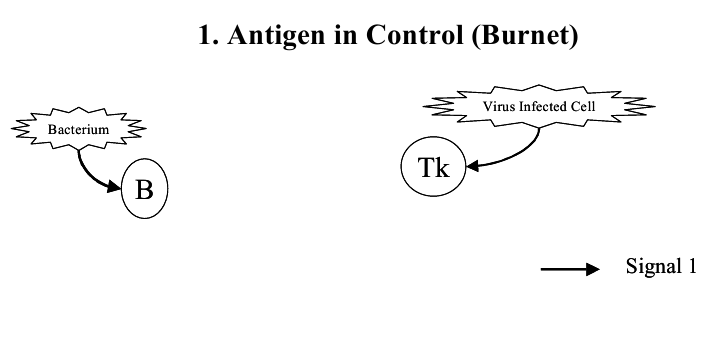
\includegraphics[width=0.75\textwidth]{img/signals1-antigen.png}
    \caption{SNSD: Antígeno no controle \cite{Aickelin2002}}
    \label{img:signals-first}
    \vspace{1cm}
\end{figure}

Em algum ponto no início da vida os linfócitos aprendem a diferenciar o próprio, células pertencentes ao corpo, do não-próprio, células estranhas ao corpo, que devem ser eliminadas. As células que geram respostas auto-imunes (reações contra as células próprias) são removidas nesse ponto, restando apenas as capazes de identificar o não-próprio.

\begin{figure}[h!]
    \vspace{1cm}
    \centering
    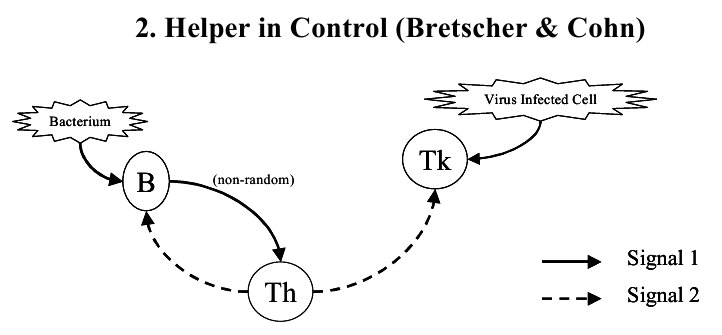
\includegraphics[width=0.75\textwidth]{img/signals2-helper.png}
    \caption{Auxiliar no controle \cite{Aickelin2002}}
    \label{fig:nis_helper}
    \vspace{1cm}
\end{figure}

Mais tarde, Bretscher e Cohn introduziram uma segunda célula, o linfócito T auxiliar, ou T$_{h}$ (T \emph{helper}), que regulava a ativação dos linfócitos B (figura \ref{fig:nis_helper}). O linfócito B apresenta o antígeno ao linfócito T e aguarda sua confirmação para iniciar a resposta. A introdução dessa célula tem o objetivo de evitar uma reação auto-imune sem controle. Lafferty e Cunningham introduziram uma terceira célula, a Célula Apresentadora de Antígeno (APC, \emph{Antigen Presenting Cell}), cuja função é decompor os antígenos e apresentá-los aos linfócitos T. Dessa forma, o funcionamento das células do modelo anterior agora depende da ativação do linfócito T pela APC (figura \ref{fig:nis_apc}).

\begin{figure}[h!]
    \vspace{1cm}
    \centering
    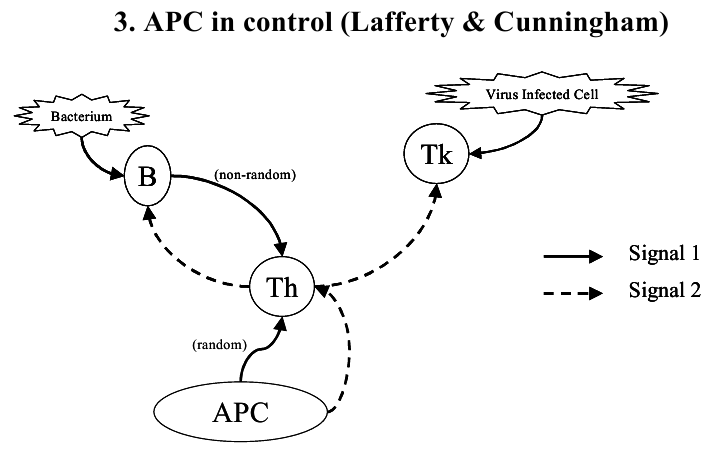
\includegraphics[width=0.75\textwidth]{img/signals3-apc.png}
    \caption{APC no controle \cite{Aickelin2002}}
    \label{fig:nis_apc}
    \vspace{1cm}
\end{figure}

\section{Não-próprio infeccioso}

O modelo mais aceito na imunologia atualmente é o modelo não-próprio infeccioso (Infectious Non-Self, INS), que foi proposto por Janeway \cite{Janeway1989}. Nele, as APCs também têm de ser ativadas: elas só enviam o sinal dois aos linfócitos T quando tiverem reconhecido padrões patológicos no antígeno (figura \ref{fig:nis_nsinf}). Assim, da mesma forma que no modelo anterior, o funcionamento de todo o sistema depende de um fator externo. No modelo anterior, a APC ativava o sistema, no modelo de Janeway, a APC tem que ser ativada através do reconhecimento de padrões no antígeno, e então ativar o sistem.

\begin{figure}[h!]
    \vspace{1cm}
    \centering
    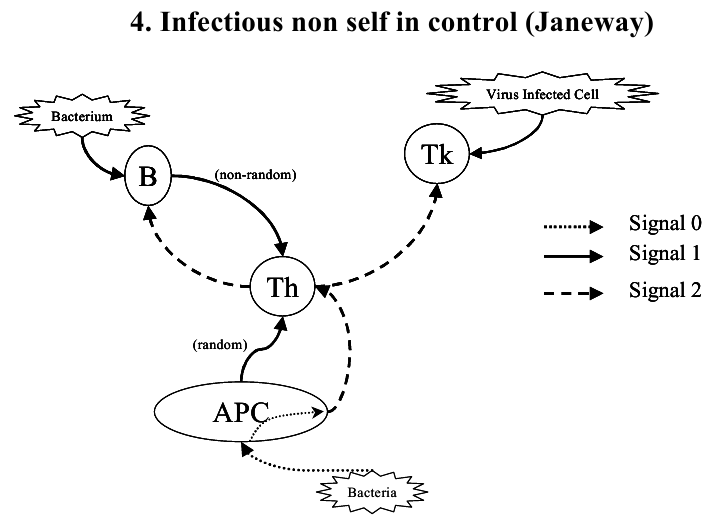
\includegraphics[width=0.75\textwidth]{img/signals4-ins.png}
    \caption{INS: Não-próprio infeccioso no controle \cite{Aickelin2002}}
    \label{fig:nis_nsinf}
    \vspace{1cm}
\end{figure}

\section{A Teoria do Perigo}

Uma adição ainda mais recente foi a da Teoria do Perigo \cite{Matzinger1994}. Matzinger defende a teoria de que não é a distinção do próprio e do não-próprio a força que impulsiona o sistema imunológico, mas sim o que ela caracteriza como ``perigo'': qualquer coisa que cause estresse ou morte não-apoptética (não natural) da célula. A Teoria do Perigo baseia-se em sinais gerados pelos tecidos danificados para diferenciar entre eventos malignos e benignos \cite{Cayzer2007}.

Embora não seja completa, essa teoria explica fenômenos que as teorias baseadas na discriminação do próprio e não-próprio não explicavam, como o fato de não haver reação contra bactérias no intestino ou na comida, a mudança do conceito de próprio durante a vida e a problemática da própria definição do próprio e do não-próprio.

Mais do que isso, a Teoria do Perigo muda a forma como se enxerga o sistema imunológico como um todo: um sistema responsável por manter o corpo em estado de equilíbrio. Dessa forma, a distinção explícita do próprio se torna desnecessária. Discriminação ainda existe, mas seu foco é o perigo, não mais o estranho.

Uma explicação detalhada do sistema imunológico, e seu funcionamento conforme a Teoria do Perigo, é apresentado na figura \ref{img:nis_danger}. Os linfócitos B são os responsáveis pela identificação de antígenos através de receptores em sua superfície. Durante uma infecção, essas células se multiplicam e produzem anticorpos para eliminar os antígenos identificados. Elas são capazes de adaptar-se a virtualmente qualquer tipo de antígeno, gerando a resposta adequada. Um outro tipo de linfócito, os linfócitos T, quando ativados, podem exercer uma de duas funções: os linfócitos T citotóxicos (CTL) são responsáveis pela eliminação de células infectadas, enquanto que os linfócitos T auxiliares (T$_{h}$) são responsáveis pela ativação de outras células, entre elas os linfócitos B.

Além disso, alguns linfócitos T são mantidos como células de memória. Durante a resposta imunológica, os linfócitos B e T$_{h}$ se multiplicam para combater os antígenos e são removidos quando a resposta termina. No entanto, alguns linfócitos T são mantidos, para que possam ser usados em futuras respostas ao mesmo tipo de antígeno. A combinação de linfóctios T virgens (sem um tipo de antígeno associado) e de memória permite que o sistema imunológico gere respostas tanto a novas ameaças quanto a ameaças recorrentes.

Existe ainda um outro tipo de linfócito, o T \emph{killer} (T$_{k}$), que não tem receptores antígeno-específicos, mas é capaz de reconhecer células infectadas e algumas células anormais. O objetivo dessas células é atuar como a primeira defesa contra infecções, e são muito importantes nos começo da vida.

\begin{figure}[h!]
    \vspace{1cm}
    \centering
    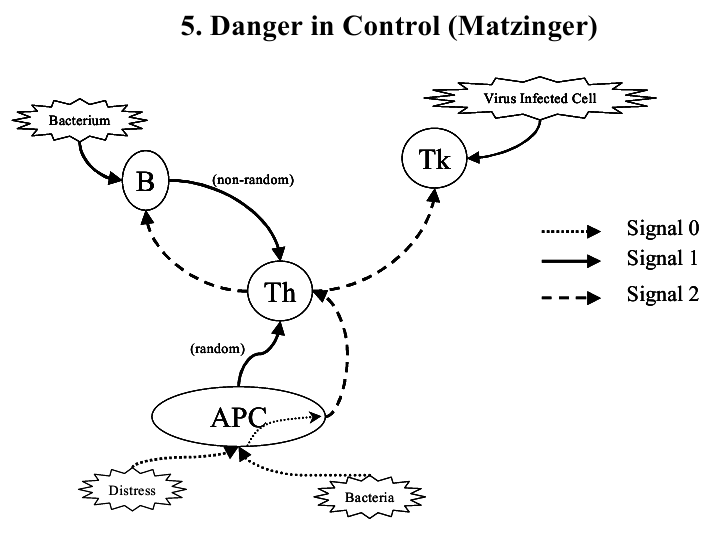
\includegraphics[width=0.75\textwidth]{img/signals5-danger.png}
    \caption{Perigo no controle \cite{Aickelin2002}}
    \label{img:nis_danger}
    \vspace{1cm}
\end{figure}

O comportamento dos linfócitos T e B se baseia em três regras:

\begin{enumerate}[a)]
\item Linfócitos T e B entram em atividade ao receber os sinais um e dois, morrem ao receber apenas o sinal um e ignoram o sinal dois sem o recebimento do sinal um.
\item Linfócitos T aceitam o sinal dois apenas de APCs, enquanto os linfócitos B, apenas de linfócitos T ativos ou células de memória. O sinal um pode ter origem em qualquer célula.
\item Linfócitos T ativados não precisam do sinal dois para entrarem em ação. Após um período de tempo, eles voltam ao estado de repouso, necessitando novamente dos dois sinais.
\end{enumerate}

Células Apresentadoras de Anítgeno são as células responsáveis por apresentar os antígenos às células T. Essas células podem ser os linfócitos B, macrófagos e as células dendríticas. Quando as células se encontram em estado de estresse ou morrem de forma não programada, enviam um sinal para as células APC, representado pela seta Sinal 0 (figura \ref{img:nis_danger}. Isso desencadeia o envio do sinal dois para os linfócitos T$_{h}$. Enquanto isso, linfócitos B usam seus receptores para reconhecer antígenos nas suas redondezas, enviando o sinal um para os linfócitos T$_{h}$. É o par de sinais um (reconhecimento do antígeno) e dois (sinal enviado pelo linfócito T, ativado pelo sinal de perigo) que faz com que a reação imunológica tenha início.

Um conceito importante da Teoria do Perigo é a tolerância. Linfócitos B que reconhecem células próprias continuamente recebem o sinal um (identificação através dos receptores em sua superfície). No entanto, essas células não apresentam perigo (não causam danos a outras células), logo o sinal dois nunca será gerado. Sem receber o sinal dois de outras células, o linfócito será removido, conforme a primeira regra das três regras apresentadas acima. Dessa maneira, corpos estranhos mas que não causem dano (perigo) ao corpo não geram respostas imunes.

\section{Considerações finais}

A imunologia como ciência existe desde o século 18, e o sistema imunológico ainda é uma grande fonte de pesquisa, em particular a natureza distribuída de seus mecanismos de memória, auto-tolerância e controle descentralizado. Baseando-se no funcionamento do sistema imunológico biológico, foram criados Sistemas Imunológicos Artificiais: algoritmos, estruturas e sistemas computacionais que inspiram-se nos modelos do sistema imunológico. Esses sistemas podem ser usados por imunologistas para explanação, experimentação ou previsão de situações que seriam difíceis ou impossíveis de serem reproduzidas em testes de laboratório \cite{Garrett2005}. Essa técnica é conhecida como ``imunologia computacional''.

No entanto, a maioria dos modelos de Sistemas Imunológicos Artificiais também são utilizados como abstrações dos processos imunológicos para o desenvolvimento de sistemas computacionais. O sistema imunológico é um sistema adaptativo complexo, que evoluiu nos seres vertebrados para protegê-los de invasores. O objetivo do estudo dos Sistemas Imunológicos Artificiais é aplicar na concepção de sistemas computacionais estruturas e funcionalidades inspiradas nos modelos biológicos. A importância dos Sistemas Imunológicos Artificiais é definida da seguinte forma \cite{Dasgupta2006}:

\begin{quote}
    Do ponto de vista do processamento de informação, o sistema imunológico é um sistema adaptativo notavelmente paralelizado e distribuído com um mecanismo de controle (parcialmente) descentralizado. Ele usa extração de características, sinalização, aprendizagem, memória e recuperação associativa para solucionar tarefas de reconhecimento e de classificação. Em particular, ele aprende a reconhecer padrões relevantes, lembrar padrões que foram já foram vistos e usar análise combinatória para construir detectores de padrão eficientes. Além disso, o funcionamento do sistema como um todo é uma propriedade emergente de muitas interações locais. Essas notáveis habilidades de processamento de informações do sistema imune representam aspectos importantes no campo da computação. \cite{Dasgupta2006}\footnote{``From an information-processing perspective, the immune system is a remarkable parallel and distributed adaptive system with (partial) decentralized control mechanism. It uses feature extraction, signaling, learning, memory, and associative retrieval to solve recognition and classification tasks. In particular, it learns to recognize relevant patterns, remember patterns that have been seen previously, and use combinatorics to construct pattern detectors efficiently. Also, the overall behavior of the system is an emergent property of many local interactions. These remarkable information-processing abilities of the immune system provide several important aspects in the field of computation.''\cite{Dasgupta2006}}
\end{quote}

Durante a história da Inteligência Artificial, os modelos biológicos inspiraram muitos modelos de algoritmos imunológicos. Tipos diferentes de modelos podem ser utilizados em domínios diferentes de problemas e existem modelos que podem ser aplicados em mais de um domínio. Dentre estes modelos, destacam-se o algoritmos de seleção negativa, as redes imunológicas artificiais, o algoritmo de seleção clonal, os algoritmos genéticos e os baseados na Teoria do Perigo. As definições, características, funções e implementações desses sistemas são apresentadas no capítulo seguinte.

\chapter{Sistemas imunológicos artificiais}

O estudo sobre os Sistemas Imunológicos Artificiais (um subcampo da área de Inteligência Computacional) iniciou no início dos anos 90, baseado na proposição de aplicar modelos teóricos da Imunologia a problemas de aprendizagem de máquina e automação.

Os primeiros trabalhos basearam-se em paradigmas como o das Redes Imunológicas Artificiais, os Algoritmos Genéticos, Aprendizagem por Reforço e Sistemas de Classificação. Os primeiros trabalhos a formarem uma identidade própria desses algoritmos foram aqueles que relacionavam o sistema imunológico como uma analogia aos sistemas computacionais de proteção da informação, como \citet{Forrest1994} e \citet{Forrest1997}.

Os algoritmos modernos são inspirados em algoritmos de três campos principais: seleção clonal, seleção negativa e redes imunológicas. Esse tipo de sistema é comummente aplicado a problemas de detecção de padrões, classificação, otimização, \emph{clustering} e outros domínios de aprendizagem de máquina.

A última década mostrou um grande aumento no interesse pelos algoritmos baseados em sistemas imunológicos, conforme apresentado em \citet{Dasgupta2010}, por serem uma boa fonte de inspiração para novas abordagens para solução de problemas complexos. O sistema imunológico natural oferece metáforas ricas pelo fato de ser um sistema altamente distribuído, adaptativo e auto-organizável, além de suas capacidades de aprendizado, memorização, extração de características e reconhecimento de padrões.

Esse artigo contém uma lista de diversos trabalhos recentes na área de Sistemas Imunológicos Artificiais. A tabela \ref{ais:recent} apresenta uma lista dos algoritmos, além do número de trabalhos apresentados.

\vspace{2mm}
\begin{table}[h!]
    \centering
    \caption{Trabalhos recentes na área de Sistema Imunológico Natural \cite{Dasgupta2010}}
    \begin{tabular}{l c r}
        \hline
        Algoritmos & Trabalhos   \\
        \hline
        Seleção negativa    & 27 \\
        Abordagens híbridas & 18 \\
        Células dendríticas & 14 \\
        Redes imunológicas  & 10 \\
        Teoria do Perigo    & 8  \\
        Seleção clonal      & 5  \\
        Outros modelos      & 3  \\
        \hline
    \end{tabular}
    \label{ais:recent}
\end{table}
\vspace{2mm}

\section{Algoritmos}

Em \citet{Dasgupta2010}, os autores apresentam pesquisas recentes na área de Sistemas Imunológicos Artificiais, e mostram que as pesquisas recentes nessa área têm se focado em quatro algoritmos principais. Esse algoritmos são: (1) seleção negativa, (2) redes imunológicas artificiais, (3) seleção clonal e (4) Teoria do Perigo e algoritmos de células dendríticas, e serão apresentados nas seções seguintes.

\subsection{Seleção negativa}

Forrest et al \cite{Forrest1994} publicou um artigo chamado "Self-Nonself Discrimination in a Computer" (Discriminação do Próprio-Não-Próprio em um Computador), que propunha um método chamado de \emph{algoritmo de seleção negativa}. Esse algoritmo é baseado na capacidade de discriminação entre o próprio e o não-próprio no sistema imunológico adaptativo através do processo de seleção negativa na geração de células T no sistema imunológico. Foi projetado para aplicações de detecção de alteração, detecção de intrusão e outros problemas de reconhecimento de padrões e classificação binária, e foi aplicado inicialmente a um problema de detecção de vírus de computador.

 O princípio da técnica da seleção negativa é a modelagem do que é desconhecido como um complemento do que é conhecido. Isso é conseguido através de um processo contínuo de seleção negativa, que elimina células que reajam a células próprias. No sistema imunológico natural, as precursoras das células T deslocam-se da medula óssea para o timo, onde ocorre o seu desenvolvimento. As células proliferam-se e diferenciam-se, através de mutação genética. A seleção negativa é aplicada sobre aquelas células T que são ativadas por células próprias. Os algoritmos baseados na seleção negativa são baseados nesse comportamento, e suas principais características são a representação negativa da informação, geração distribuída do conjunto de detectores e classificação dos dados em apenas uma classe.

A representação dos dados é um dos principais aspectos desse algoritmo: geralmente são usados \emph{strings} ou vetores de valores reais. Existe também uma regra de combinação particular de cada algoritmo, tipicamente baseada em distância ou alguma medida similar. Muitas variações desse algoritmo foram desenvolvidas, mas todas compartilham essas características básicas.

\subsection{Redes imunológicas artificiais}

Redes imunológicas artificiais (\emph{Artifial immune networks}, AINs) são inspiradas no modelo de redes imunológicas de Farmer et. al \cite{Farmer1986}, e foram propostas por \cite{Ishida1990}. \cite{Timmis2000} redefiniu e reimplementou a rede imunológica artificial, e esses trabalhos foram nomeados conjuntamente como AINEs (\emph{Artificial Immune NEtworks}, Rede Imunológicas Artificiais). Uma rede imunológica artificial consiste de um conjunto de células B e ligações entre essas células. Essas redes permitem ao sistema imunológico ter uma memória imunológica: as células estimulam ou reprimem umas às outras, atingindo uma memória estável. Sua utilização é ampla em campos como a mineração de dados e aprendizagem de máquina. 

O sistema proposto por \citeauthor{Timmis2000} era composto de uma medula óssea, uma rede de células B e uma população de antígenos. A população de células B é inicializada aleatoriamente e, uma a uma, são inseridas em um ponto também aleatório na rede. Caso a célula seja capaz de ligar-se à população de antígenos, clones das células B são gerados, e aqueles com maior afinidade com as células da rede são mantidos. Os algoritmos de redes imunológicas artificiais incorporaram algumas ideias das teorias da seleção clonal: as células B nas AINE sofrem clonagem, mutação e seleção quando são estimuladas pela rede.

\subsection{Seleção clonal}

Em 2000, Castro et al.\cite{Castro2000} propôs o algoritmo de seleção clonal (CSA), mais tarde conhecido como CLONALG. Esse algoritmo é baseado nos princípios da imunidade adquirida de seleção clonal e maturação de afinidade, que são por sua vez baseados nos princípios da teoria de Darwin da seleção natural.

Segundo a teoria da seleção clonal, quando um linfócito identifica um antígeno, ele prolifera, criando milhares de cópias de si mesmo, e diferenciando-se em diferentes tipos de células: de plasma e de memória.

Células de plasma têm vida curta, e produzem grandes quantidades de anticorpos moleculares. Células de memória vivem por um longo período, fazendo parte das respostas secundárias caso o antígeno venha a ser identificado novamente.

A clonagem de células B causam um aumento na afinidade do antígeno que causou a clonagem, através de um processo denominado maturação de afinidade. Esse processo é composto de duas partes: hipermutação somática, que diversifica os anticorpos introduzindo mudanças aleatórias nas novas gerações; e um mecanismo de seleção, que garante que apenas os clones com maior afinidade sobrevivam. Assim, uma geração de células inclui a inicialização de soluções candidatas, seleção, clonagem, mutação, reseleção e substituição de população, semelhante a um algoritmo genético (GA).

A parte essencial dessa teoria é que, quando um linfócito é clonado, sofre pequenas alterações em sua estrutura (hipermutação somática), que alteram seus receptores e sua capacidade de reconhecimento, assim como os anticorpos que são gerados por ele. Assim, essa teoria sugere que um repertório inicial de células imunes genéricas é capaz de evoluir para responder a mudanças no ambiente, sem ter informações detalhadas sobre os agentes que compõem esse ambiente.

\subsection{Teoria do Perigo}

No primeiro artigo a propor a aplicação da Teoria do Perigo em um sistema computacional, \citeauthor{Aickelin2002} apresentam como a Teoria do Perigo pode auxiliar na aplicação de sistemas imunológicos artificiais em problemas complexos de detecção de anomalia, citando algumas analogias dos sistemas imunológicos presentes na Teoria do Perigo:

\begin{enumerate}[a)]
    \item Uma APC é necessária para apresentar o sinal de perigo.
    \item O "sinal de perigo" pode não ter relação nenhuma com perigo.
    \item O sinal de perigo pode ser positivo (presença de sinal) ou negativo (ausência de sinal).
    \item Uma medida de proximidade pode ser usada para simular uma zona de perigo.
    \item Uma resposta imunológica não deve gerar novos sinais de perigo.
\end{enumerate}

Segundo a teoria do perigo, a resposta imunológica é desencadeada por sinais de perigo. Representações dos sinais de perigo podem incluir uso anormal de memória, atividade de disco imprópria, etc. O sistema imunológico reage aos antígenos dentro de uma zona de perigo centrada no local da origem do sinal, que pode ser modelada como uma medida de similaridade ou relação de causalidade. Aqueles anticorpos que combinam-se aos antígenos (sinal um) dentro de uma zona de perigo (sinal dois) proliferam, gerando células de memória.

\subsection{Algoritmo de células dendríticas}

O algoritmo de células dendríticas é inspirado pela Teoria do Perigo, mais especificamente na função das células dendríticas. As células dendríticas foram identificadas por \citet{Steinman1973} e o seu principal papel é o de célula apresentadora de antígeno (APC). O objetivo do algoritmo de células dendríticas é preparar um conjunto de células dendríticas maduras que forneçam informações dependentes de contexto sobre como classificar como normais ou anômalos os padrões de entrada.

As células dendríticas encontram-se distribuídas em todos os tecidos e executam funções diferentes de acordo com o tecido em que atuam. Quando ainda estão em um estado de imaturidade viajam na corrente sanguínea, até que sofrem diferenciação e maturação quando propriamente estimuladas. Elas então migram para tecidos periféricos, onde apresentam antígenos para as células T, iniciando as respostas imunológicas. As células dendríticas são de três tipos principais:

\begin{description}
    \item[Imaturas]: coletam partes dos antígenos e sinais
    \item[Semi-maduras]: decidem que os sinais locais não representam perigo e apresentam um sinal de tolerância às céulas T
    \item[Maduras]: decidem que os sinais locais são de perigo e apresentam um sinal de reposta imune às células T
\end{description}

O primeiro algoritmo baseado no comportamento dessas células foi desenvolvido em \citet{Greensmith2005} e definido formalmente em \citet{Greensmith2006}. Esse algoritmo combina sinais múltiplos para estimar o estado corrente do ambiente e amostrar outro antígeno assincronamente. Sua execução consiste de três etapas principais: inicialização, atualização e agregação. A inicialização configura diversos parâmetros. A fase de atualização é dividida em uma fase de atualização do tecido, onde o valor dos sinais é calculado de acordo com os dados de entrada, resultando nos sinais de entrada das células, e uma fase de atualização das células. O último estágio da execução é a agregação: os antígenos coletados são analisados e classificados.

O algoritmo aplica pesos pré-definidos aos sinais de entrada para produzir três sinais de saída: sinal de coestimulação, sinal de semi-maturação e sinal de maturação. Se a soma dos valores dos sinais de maturação for maior que a somas dos sinais de semi-maturação, a célula é diferenciada para um estado maduro e tem assinalado um valor de contexto. O algoritmo calcula a proporção de valores de contexto maduro de um antígeno para o total de antígenos, chamada de MCAV (\emph{Mature Context Antigen Value}, Valor de Contexto Maduro do Antígeno), e aquelas antígenos cujo MCAV excede um limite pré-definido são classificados como anômalos.

\section{Implementação}

A modelagem de um problema como um sistema imunológico artificial requer a definição de quatro componentes: codificação, medida de similaridade, seleção e mutação. De maneira geral, o funcionamento de um sistema baseado no modelo imunológico é: uma vez que a \emph{codificação} e uma \emph{medida de similaridade} tenham sido escolhidas, o sistema executa a \emph{seleção} e \emph{mutação}, ambas baseadas na medida de similaridade, até que o critério de parada seja satisfeito \cite{Aickelin2005}. Essas quatro etapas são detalhadas nas próximas seções.

\subsection{Codificação}

A codificação é uma etapa essencial na definição de um Sistema Imunológico Artificial. Ela afeta toda modelagem do sistema, em especial a medida de similaridade, e pode ser responsável pelo seu sucesso ou falha. Os dois principais agentes do sistema imunológico, antígenos e anticorpos, são também os principais elementos que devem ser modelados. Eles são são comumente representados da mesma forma.

Um antígeno é uma parte do objetivo ou solução da aplicação, que pode ser único ou um parte de um conjunto-solução. Os anticorpos são o resto dos dados, e geralmente existem em grande quantidade. Em uma aplicação de detecção de intrusão, por exemplo, o antígeno poderia ser o conjunto de dados que define um tráfego de dados, e os anticorpos, os conjuntos de dados que já foram identificados como legais.

Na maioria dos problemas, a representação desses dois elementos é feita através de um vetor de números ou de características. Cada posição desse vetor representa uma característica da instância. Os tipos mais comuns de dados são números (inteiros ou reais), \emph{strings} e valores binários.

\subsection{Medida de similaridade}

A medidade de similaridade (também chamada de medida de afinidade, principalmente na área de Sistemas Imunológicos Artificiais) é usada para comparar duas instâncias, e mede o quanto uma é semelhante à outra. É usada principalmente para agrupar instâncias em grupos e nas condições de término (o algoritmo termina quando o modelo descreve as instâncias com uma medida de similaridade satisfatória, que varia de acordo com a aplicação, o tempo de execução e o nível de similaridade necessário).

Uma função de similaridade simples é o número de \emph{bits} que são idênticos nas duas sequências. Por exemplo, para os \emph{strings} (00011) e (00000), a função retornaria 3. Essa função é oposta à distância de Hamming, que mede quantos \emph{bits} devem ter seus valores trocados para tornar as sequências iguais. Em alguns problemas, essa medida não é suficiente, já que ela não tem a noção de continuidade. Uma alternativa é calcular o número de posições iguais contínuas, retornando o maior valor. Assim, o exemplo anterior também receberia o valor 3, mas as sequências (00000) e (01010) receberia 1. Essa diferenciação pode ter ser apropriada ou não, dependendo do problema. Para variáveis não-binárias, existem ainda mais possibilidades de medida de distância, como a distância Euclideana.

Para os problemas de mineração de dados, a aptidão geralmente significa correlação, e uma medida simples de correlação é o coeficiente de correlação de Pearson. A correlação de duas instâncias \emph{u} e \emph{v} é definida como:

\vspace{2mm}
\begin{equation}
r=\frac{
    \sum\limits_{i=1}^{n}
        (u_i-\overline{u})
        (v_i-\overline{v})
    }
    {\sqrt{
        \sum\limits_{i=1}^{n}
            (u_i-\overline{u})^2
        \sum\limits_{i=1}^{n}
            (v_i-\overline(v))^2
        }
    }
\end{equation}
\vspace{2mm}

Onde \emph{u} e \emph{v} são duas instâncias, \emph{n} é o número de variáveis comuns a u e v, \emph{$u_i$} é o valor da varável i na instância u e \emph{$\overline{u}$} é a média dos valores de todas as variáveis de u (não apenas das variáveis comuns a u e v). A média é modificada para que o valor 0 seja atribuído a instâncias sem nenhuma variável em comum. O resultado são valores de -1 a 1, onde 1 significa forte concordância e -1 forte discordância.

Para algumas aplicações, aptidão pode não ser benéfica, e as instâncias que são mais semelhantes são na verdade descartadas. Esse processo é conhecido como seleção negativa, e é equivalente ao processo que acredita-se que ocorre durante a maturação dos linfócitos B, onde eles aprendem a não identificar os tecidos próprias, para que não se inicie uma reação autoimune.

A seleção negativa é muito aplicada a sistemas de segurança. Cria-se um ambiente seguro, formado apenas por componentes confiáveis. Na inicialização do sistema, é gerado um grande número de detectores randômicos, que são aplicados aos dados gerados por esse ambiente. Aqueles que identificarem os dados legais são eliminados, restando ao final apenas aqueles que não identificarem. Esses detectores formarão o sistema de detecção, que irá monitorar constantemente o ambiente. Caso algum detector identifique os dados no ambiente, é gerado um alerta de "possível não-próprio".

A otimização da aptidão dos modelos em muitos casos não é realmente o objetivo do sistema se o objetivo é criar generalizações através de um subconjunto dos dados existentes \cite{Hand2001}. Um modelo com grande aptidão pode não se adaptar a novas instâncias que venham a ser analisadas pelo sistema.

\subsection{Seleção}

Nos Sistemas Imunológicos Artificiais, os três métodos de seleção mais usados são a seleção negativa, seleção clonal e seleção de vizinhança. O papel da seleção é explicado a seguir, no contexto do funcionamento do sistema. O estado inicial do sistema é vazio. O antígeno é então codificado (conforme a representação definida anteriormente) e adicionado ao sistema. Cada anticorpo é codificado e adicionado ao sistema, um a cada iteração. Os anticorpos iniciam com um determinado valor de concentração, que é análogo ao número de células presentes no sistema imunológico artificial. Esse valor é constantemente decrementado conforme o tempo passa, representando a morte natural de parte das células.

Anticorpos cuja concentração ultrapassa um certo limiar mínimo são removidos do sistema. Um anticorpo aumenta sua concentração de acordo com a sua similaridade com o antígeno. Quanto maior a similaridade, mais sua concentração aumenta, em um processo similar à expansão clonal que ocorre com as células imunológicas quando identificam um antígeno. Após todos os antígenos serem adicionados ao sistema, começa um processo iterativo de decremento de concentração e clonagem, até que o sistema entre em equilíbro: não ocorram remoções por um determinado período de tempo.

O trecho de código \ref{aisalg} mostra o pseudocódigo de um Sistema Imunológico Artificial.

\begin{lstlisting}[caption=Pseudo código de um Sistema Imunológico Artificial \cite{Aickelin2005},label=aisalg]
Inicializar o sistema
Codificar o antígeno Ag
ENQUANTO (Sistema não cheio) E (Ainda existem anticorpos) FACA
    Adicionar próximo anticorpo Ab
    Calcular a medida de similaridade entre Ag e Ab
    ENQUANTO (Sistema cheio) E (Sistema não estabilizado) FACA
        Reduzir a concentração de todos os Abs
        Estimular os Abs conforme a medida de similaridade
    FIMENQUANTO
FIMENQUANTO
\end{lstlisting}

\subsection{Mutação}

A mutação utilizada nos sistemas imunológicos é similar àquela encontrada em Algoritmos Genéticos. \emph{Strings} binárias têm seus dígitos invertidos, valores reais são alterados aleatoriamente e os outros tipos são trocados de posição. Além disso, geralmente usa-se a mutação somática, inspirada na reprodução de células do sistema imunológico, onde a mutação é mais severa conforme o grau de similaridade entre o anticorpo e o antígeno aumenta (ou diminui, caso esteja-se aplicando a seleção positiva). 

A estratégia de mutação deve ser planejada com cuidado, porque nem todas as técnicas funcionam para qualquer tipo de dados. \citet{Aickelin2005} utiliza o exemplo de um sistema de recomendação de filmes, onde uma base de dados é utilizada para recomendar filmes aos usuários, analisando usuários que recomendaram filmes semelhantes àqueles recomendados por ele. Nesse caso, não faria sentido aplicar algum tipo de mutação: ao fim, os anticorpos convergiriam para o próprio usuário.

Mesmo assim, a mutação pode ser muito útil quando aplicada a alguns problemas, como detecção de intrusão e mineração de dados \cite{DeCastro2002}. 

\section{Espaço de formas}

Os formalismos do espaço de formas e topologia de afinidade são dois paradigmas geométricos populares, originados na imunologia teórica e computacional, muito utilizados em aplicações recentes do campo de sistemas imunológicos artificiais \cite{Brownlee2007}. \citeauthor{Perelson1979} apresentaram o formalismo do espaço de formas em \citet{Perelson1979}, onde os autores fizeram uma investigação teórica das diferentes formas e capacidades de reconhecimento dos anticorpos. As ideias apresentadas nesse trabalho influenciara muitos trabalhos no fim dos anos 80 e início dos anos 90, principalmente em trabalhos teóricos sobre seleção clonal e redes imunológicas.

Dados um anticorpo \emph{ab} e um antígeno \emph{ag}, é criado um vetor onde as características relacionadas à ligação entre esses dois são discretizadas e transformadas em valores reais. Os parâmetros no trabalho original representavam características físicas, como a estrutura geométrica, carga eletrostática, entre outras. Assim, a interação \emph{ab-ag} pode ser definida como um ponto em um espaço vetorial Euclidiano \emph{S} de \emph{n} dimensões, onde \emph{n} é o número de características que compõem o vetor. Uma representação do espaço de estados, adaptada de \citet{Brownlee2007} é apresentada na Figura \ref{img:space}.

\begin{figure}[h!]
    \centering
    \caption{Diagrama do formalismo do espaço de estados \cite{Brownlee2007}}
    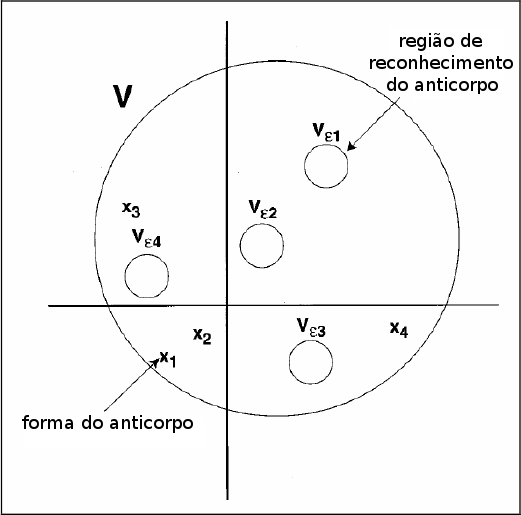
\includegraphics[width=0.75\textwidth]{img/space.png}
    \label{img:space}
\end{figure}

O espaço de formas é um hipercubo de volume V, e cada anticorpo é definido como uma área de reconhecimento nesse espaço ($\epsilon$). Na definição original, essas áreas de reconhecimento eram funções Gaussianas. A distância euclidiana entre \emph{ab} e \emph{ag} é considerada como a `afinidade' ou `medida de complementaridade'. Para isso, a natureza complementar dos anticorpos e antígenos é ignorada: uma ligação perfeita é considerada quando \emph{ab == ag}, ao contrário de \emph{ab != ag}. Anticorpos possuem uma hiper-região de reconhecimento, onde antígenos podem gerar uma resposta imune.

Uma crítica ao formalismo do espaço de formas foi feita em \citet{Carneiro1994}, destacando principalmente a simplicidade da abstração do espaço de estados e as limitações das funções de afinidade simples.

\section{Topologia de afinidade}

O objetivo de um anticorpo, no sistema imunológico, é maximizar a sua afinidade com um antígeno específico. Assim, a maturação de um anticorpo pode ser considerada também geometricamente como uma movimentação na superfície da função de afinidade para um antígeno específico \cite{Brownlee2007}.

Essa superfície teórica é geralmente considerada como contínua, e possui diversos ótimos locais, ou seja, um ponto com maior afinidade que seus vizinhos, mas que não é o ponto global com maior afinidade. Esse formalismo é útil na definição e formalização do processo de maturação por hipermutação dos anticorpos, parte principal dos algoritmos baseados na teoria da seleção clonal.

Os formalismos do espaço de formas e topologia de afinidades são a base da definição do espaço de formas binário usado na seleção negativa e nas redes imunológicas, das regiões e limiares de detecção nos algoritmos de mineração de dados e classificação, e da movimentação na topologia das funções de custo nos algoritmos de otimização.

A interpretação geométrica genérica proporcionada por esses dois formalismos constitui um \emph{framework} para a investigação de princípios imunológicos, não limitada aos problemas de reconhecimento de padrões.

\section{Considerações finais}

\citet{Dasgupta2010} observam que a maioria dos trabalhos recentes na área de Sistemas Imunológicos Artificiais têm seu foco em aplicações, ao invés de extensões, dos algoritmos existentes. Destacam também que existe uma sobreposição entre os modelos desses algoritmos e os evolucionários: os algoritmos de redes imunológicas artificiais, seleção clonal e genéticos têm componentes importantes em comum, como a clonagem, mutação e seleção.

\chapter{Detecção de fraude}

A fraude pode ter origem tanto interna quanto externa a uma organização. Por exempo, uma empresa está sujeita a fraude por seus administradores (denominada de alto-nível) ou empregados que não sejam gestores (baixo-nível) \cite{Phua2010}. Em um documento de 2012, a Associação de Investigadores Certificados de Fraude (Association of Certified Fraud Examiners, ACFE) definiu a fraude interna como a exploração ilegal dos recursos e bens de uma empresa, por um empregado, para enriquecimento próprio \cite{ACFE2012}.

Já na fraude externa, os seus autores dividem-se em três perfis: casual, criminal e crime organizado \cite{Phua2010}. Criminosos casuais apresentam comportamento aleatório, transgredindo as leis quando têm oportunidade, tentação ou em períodos de dificuldades financeiras. Por outro lado, indivíduos ou grupos organizados são mais perigosos porque tentam esconder ou dissimular sua verdadeira identidade, além de evoluir seu \emph{modus operandi} com o tempo, tentando burlar os sistemas de detecção e evitar a sua identificação. Assim, é importante levar-se em consideração essa constante interação entre os sistemas de detecção e os fraudadores profissionais. Essas categorias de fraudadores geralmente atuam em um setor específico: as fraudes internas e de seguro são mais frequentemente exploradas por criminosos comuns, enquanto fraudes de cartão de crédito e telecomunicações são vítimas de fraudadores profissionais.

O monitoramento de sistemas com o objetivo de encontrar comportamentos fraudulentos já existia muito antes da utilização dos sistemas computacionais tornarem-se ferramentas comuns. Antes havia um processo denominado auditoria: gerar, armazenar e revisar um registro cronológico de eventos de um sistema \cite{Bace2000}. Os principais objetivos dos sistemas de auditoria são identificar os usuários do sistema, impedir o uso impróprio, e auxiliar na reconstrução de eventos e na estimativa, quantificação e qualificação de danos.

O primeiro trabalho a considerar necessária a auditoria automática de sistemas foi \citet{Anderson1972}. Nesse trabalho, Anderson classifica os riscos e ameaças a sistemas, diferenciando fontes internas e externas, como na figura \ref{fraud:and}. Ele também cita diversos objetivos para um sistema de auditoria:

\begin{enumerate}[a)]
    \item Prover informações suficientes para que o problema possa ser localizado, mas que não exponham detalhes que possibilitem um ataque.
    \item Obter dados de diversas fontes para otimizar o conteúdo do banco de dados.
    \item Discernir uma atividade ``normal'' do sistema, para que se possa detectar abusos interno.
    \item Levar em consideração as estratégias dos invasores no projeto do sistema.
\end{enumerate}

A detecção de fraude é apenas uma das etapas de um sistema chamado de \emph{controle de fraude}. Nesse contexto, a detecção automática ajuda a reduzir o trabalho manual de verificação das instâncias \cite{Phua2010}. O objetivo principal desses sistemas é identificar padrões de transações suspeitas em meio às transações comuns de uma organização. O fraudador pode, por exemplo, contratar um seguro usando informações de outra pessoa ou informações falsas. O sistema procura detectar e impedir a fraude o mais cedo possível.

\renewcommand{\arraystretch}{1.5}
\vspace{1cm}
\begin{table}[h!]
    \caption{Matriz de ameaças \cite{Anderson1972}}
    \centering
    \begin{tabular}{c p{4cm}|>{\centering\arraybackslash}p{4cm}|>{\centering\arraybackslash}p{4cm}|}
        \cline{3-4}
        & & Uso não autorizado dos dados/programa & Uso autorizado dos dados/programa \\
        \hhline{~---}
        \multicolumn{0}{c|}{} & Uso não autorizado do computador & Invasão externa & \cellcolor{gray!90} \\
        \cline{2-4}
        \multicolumn{0}{c|}{} & Uso autorizado do computador & Invasão interna & Abuso de poder \\
        \cline{2-4}
    \end{tabular}
    \label{fraud:and}
\end{table}
\vspace{1cm}

Geralmente não é possível ter absoluta certeza sobre a legitimidade das transações de um negócio a partir dos dados disponíveis. Não seria possível verificar todas as entidades com as quais uma empresa mantém relações, que em algumas empresas podem ser milhares. Assim, não existe uma técnica infalível para a detecção de fraudes. Isso não significa que elas não possam ser detectadas. A melhor alterantiva, na prática, é uma busca por possíveis evidências de fraude nos dados disponíveis. Métodos matemáticos e estatísticos são utilizados para comparar um banco de dados de transações existentes com as novas, com o objetivo de encontrar evidências de possíveis fraudes. Mesmo assim, geralmente há um processo de análise e revisão caso a caso por um especialista.

Ainda, segundo a pesquisa apresentada no mesmo trabalho, o motor analítico desse tipo de sistema pode ser composto de um ou mais métodos, tais como: Sistemas Imunológicos Artificiais, inteligência artificial, auditoria, bancos de dados, computação distribuída e paralela, econometria, sistemas especialistas, lógica nebulosa, algoritmos genéticos, aprendizagem de máquina, redes neurais, reconhecimento de padrões, estatística, visualização, entre outros.

Dois conceitos relacionados à detecção em geral são falsos positivos e falsos negativos. Falsos positivos são instâncias erroneamente classificadas, por exemplo, uma transação comum que é classificada como fraudulenta. Falsos negativos são o oposto: uma transação fraudulenta que é classificada como comum. O número de falsos positivos aumenta o trabalho desnecessário na fase de revisão, enquanto os falsos negativos reduzem a eficácia da detecção.

A redução dos falsos positivos é um dos objetivos principais de um sistema de detecção. Os falsos negativos, no entanto, são quase impossíveis de serem eliminados completamente, em qualquer sistema de detecção \cite{Michie1994}. Mesmo um sistema capaz de reconhecer sinais de fraudes existentes não é suficiente para um ambiente real. Fraudadores tentam constantemente superar os sistemas de detecção, evoluindo o se \emph{modus operandi} com o tempo, novos métodos são criados, novos fraudadores entram em atividade. Um sistema que almeje deter o maior número possível deve ser constantemente atualizado para se adaptar às mudanças de um ambiente tão dinâmico.

Dependendo do domínio da organização, para que um sistema possa prever fraudes com antecedência suficiente para que elas sejam evitadas, ele deve monitorar constantemente as novas transações em andamento. Esse fator reduz a utilização de sistemas que necessitam de um longo tempo de treinamento ou de análise. O ideal seria que ele estivesse em constante execução, analisando as transações conforme elas ocorrem. Para aplicações grandes ou descentralizadas, pode ser muito difícil conseguir isso sem afetar a performance geral das transações.

Para cada domínio, tipos diferentes de fraude podem existir, e mais de um tipo pode ocorrer simultaneamente, sem uma ordem definida. 

\section{Dados}
\label{fraud:data}

Os atributos das instâncias em um banco de dados usado para detecção de fraude geralmente limitam-se a valores binários, numéricos, categóricos ou uma mistura desses três. Os atributos específicos usados geralmente são semelhantes. Aplicações de seguro utilizam o histórico do cliente: tempo de contrato, histórico e total de pagamentos, lucro anual valor médio depositado em conta bancária. Para fraudes de crédito, utilizam-se informações sobre as transações: valor, data, localização geográfica, conta de destino, tempo de conta, etc. Fraudes em seguros de automóveis utilizam valores binários para atributos como acidente e tratamento hospitalar, além de dados do motorista, custo, tipo de ferimento, etc.

O número de instâncias positivas nas bases de dados de fraude é geralmente muito reduzido: as fraudes representam um percentual muito pequeno em relação ao número de transações legítimas de uma organização, geralmente menor do que 20\%. Métodos de detecção de fraude nunca são perfeitos: deve existir um mecanismo para lidar com as fraudes que não são identificadas a tempo de serem impedidas.

A obtenção de bancos de dados reais para teste é difícil, já que empresas e organizações, por razões legais e competitivas não disponibilizam informações desse tipo. Assim, é difícil encontrar bases de dados públicos para que os testes sejam realizados. Outra desvantagem comumente encontrada nesses bancos de dados é o fato dos dados estarem alterados, para a preservação da confidencialidade dos clientes das empresas fornecedoras. Apesar dos dados ainda poderem ser utilizados normalmente em ambientes de teste, nao é possível, como seria caso se tivesse acesso aos dados originais, derivar regras de classificiação dos resultados dos testes. Por exemplo, observando os resultados, seria possível perceber que um valor alto em um atributo leva a instância ser classificada como fraudulenta na maioria dos casos. Em uma base de dados esse atributo teria uma descrição informativa, mas isso é perdido em uma base alterada, onde ele seria descrito por um identificador sem significado, como ``atributo 5''.

Uma alternativa é a criação de um banco de dados artificial, inspirado em dados reais. A eficácia dessa técnica é limitada pela capacidade do criador do banco em prever o maior número de casos possíveis, o que geralmente é muito inferior à variedade das situações reais. Mesmo assim, essa técnica é comumente empregada na fase de concepção e teste, devido à dificuldade de obtenção de dados.

\section{Implementação}

A maioria dos sistemas de detecção de fraude opera usando listas negras (\emph{black-lists}) de dados (transações, contas, etc.), que são comparadas com as nova instâncias. Algumas utilizam regras fixas para a classificação. A figura \ref{fig:fraud-data} mostra a organização dos dados nesses sistemas. Uma parte do banco de dados é usada para o treinamento. Esses são os dados onde o sistema aprenderá os padrões e regras utilizados para a detecção. O restante das instâncias é usada para a avaliação do treinamento. Também é comum que haja bancos de dados distintos para o treinamento e avaliação.

\begin{figure}[h!]
\centering
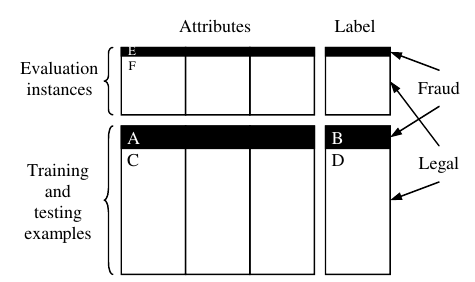
\includegraphics[width=0.75\textwidth]{img/fraud-data.png}
\caption{Dados para a análise}
\label{fig:fraud_data}
\end{figure}

A maioria dos estudos relacionados à detecção de fraude considera a detecção de \emph{outliers} como uma ferramenta principal de detecção \cite{Aral2011}. Existem muitos métodos aplicados à detecção de fraude: auditoria, sistemas especialistas, lógica nebulosa (\emph{fuzzy}), redes neurais, reconhecimento de padrões, árvores de decisão, regressão, etc \cite{Huang2010}. Considerando os dados dividos conforme a figura \ref{fig:fraud_data}, as duas técnicas mais usadas são:

\begin{enumerate}[a)]
\item Dados para treinamento classificados (A + B + C + D) processados por um algoritmo supervisionado.
\item Instâncias legais (C) processadas por um algoritmo semi-supervisionado.
\end{enumerate}

Algoritmos supervisionados examinam as instâncias previamente classificadas (A + B + C + D) para identificar matematicamente os padrões presentes nas classificadas como fraudulentas. Os algoritmos mais utilizados nessa categoria são as redes neurais. Outros algoritmos incluem máquinas de vetores de suporte (\emph{support vector machine}, SVM), árvores de decisão e raciocínio baseado em casos. Para aumentar a eficácia dos métodos supervisionados, esses algoritmos podem ser aplicados em sequência. Também podem ser combinados resultados de bancos de dados distintos.

Algoritmos não-supervisionados atuam sobre dados não classificados (A + C + E + F), e o seu objetivo é agrupar os dados em padrões, para que estes sejam mais facilmente analisados, combinando a detecção humana e a computação da máquina. Exemplos desses algoritmos são redes neurais não supervisionadas, análise de ligações (\emph{link analysis}) e mineração de grafos (\emph{graph mining}).

A combinação de dois ou mais algoritmos supervisionados, ou de algoritmos supervisionados e não-supervisionados, chamados de algoritmos híbridos, é uma grande área de pesquisa. Também são utilizados algoritmos supervisionados em bancos de dados que contêm apenas instâncias legais (C). Regras são geradas e testadas na base de dados, e aquelas que identificam padrões nesses dados são descartadas. Esses algoritmos são chamados de semi-supervisionados, porque apesar de não fazerem distinção entre dados legais e ilegais, os dados ainda necessitam ser classificados para que sejam utilizados no seu treinamento.

Autores como Phua fazem muitas críticas ao uso de dados previamente classificados para o treinamento dos sistemas \cite{Phua2010}. A classificação atrasa o processo de detecção, aumenta o tempo de reação a novos tipos de fraudes e pode ser cara e difícil de se obter. Pode ainda ser incorreta, tendenciosa e expor dados sigilosos, dependendo do tipo de aplicação. Assim, instâncias de treinamento e avaliação (A + C + E + F, sem classificações) devem ser combinadas e processadas por um algoritmo não-supervisionado, detectando regras, pontuações ou anomalias visuais nos dados avaliados.

Um sistema que detecte e reporte uma fraude muito tempo depois de ela ter ocorrido permite que o fraudador consiga causar um dano substancial. Em geral, esse tempo de resposta de um sistema a partir do momento em que uma fraude é concretizada até a sua detecção é crucial para a eficácia do sistema em de fato proteger o ambiente em que é inserido.

Os sistemas de detecção podem ser divididos em dois tipos gerais, denominados \emph{on-line} e \emph{off-line}, enquanto alguns incorporam características dos dois modelos e outros têm um processo distinto para ambos, que interagem entre si para gerar o resultado final.

\iffalse

\cite{Huang2010}.

\fi

\section{Critérios de avaliação}
\label{sec:fraud_criteria}

Phua e outros autores listam as diversas medidas de performance utilizadas em trabalhos recentes na área de detecção de fraude \cite{Phua2010}. Os métodos tradicionais de medição, como a taxa de positivos (número de fraudes detectadas corretamente dividido pelo número de fraudes verdadeiras) e a precisão a um determinado limite (número de instâncias classificadas corretamente, dividido pelo número total de instâncias) foram abandonados pelos trabalhos recentes, devido à natureza peculiar da detecção de fraude.

A razão para isso é que o custo das classificações errôneas, no caso da detecção de fraude, são irregulares, incertos, variam de exemplo a exemplo e podem variar conforme o tempo. Falsos negativos são geralmente mais custosos do que falsos positivos. Um falso positivo geralmente leva apenas a uma verificação desnecessária por um especialista. Um falso negativo, no entanto, acarreta em uma fraude que não é detectada pelo sistema e não será reportada, deixando o fraudador impune. Mesmo assim, muitos dos sistemas de detecção comerciais, como a maioria dos departamentos governamentais que atuam na área de detecção de fraude, utilizam valores monetários como medida de avaliação \cite{Phua2010}.

Classificadores binários são aqueles que, para um dado conjunto de valores de entrada, geram como valor de saída um valor Booleano: verdadeiro ou falso, positivo ou negativo. Os sistemas de detecção de fraude se situam, na maioria dos casos, nessa categoria: os dados referentes a uma instância passam pelo sistema de detecção e são classificados como legítimos ou fraudulentos \cite{Bewick2004}. Sistemas mais complexos podem gerar saídas com mais informações sobre a instância, como o grau de certeza da previsão ou o grau de semelhança entre a instância e os dados da base.

A avaliação dos classificadores binários é feita com base em uma \emph{tabela de confusão}, conforme mostrado na tabela \ref{fraud:confusion}. Nessa tabela são listados o número de valores (ou porcentagem) para cada combinação de saída do sistema e a classificação real. Instâncias corretamente classificadas ocupam as colunas Positivo e Negativo, enquanto instâncias cujo classificação difere da realidade ocupam as colunas ``Falsos positivos'' e ``Falsos negativos''.

\renewcommand{\arraystretch}{1.5}
\vspace{2mm}
\begin{table}[h!]
    \caption{Tabela de confusão}
    \centering
    \begin{tabular}{c l c c}
        & & \multicolumn{2}{c}{\textbf{Dados reais}} \\
        \multirow{3}{5mm}{\begin{sideways}\parbox{20mm}{\textbf{Saída}}\end{sideways}} & \multicolumn{1}{c|}{} & Positivo & Negativo \\
        \cline{2-4}
        & \multicolumn{1}{c|}{Positivo} & Positivo & Falso positivo\\
        & \multicolumn{1}{c|}{Negativo} & Falso negativo & Negativo\\
    \end{tabular}
    \label{fraud:confusion}
\end{table}
\vspace{2mm}

Como exemplo, inspirado em \citet{Bewick2004}, é apresentado nessa seção um sistema de detecção de fraude, que considera como único atributo das instâncias o número de ocorrências de um determinado valor. Nesse ambiente simplificado, a instância é considerada fraudulenta caso um limiar de ocorrências seja ultrapassado. Um exemplo de dados presentes na base desse sistema é mostrado na tabela \ref{fraud:ex_data}.

\renewcommand{\arraystretch}{1.5}
\vspace{2mm}
\begin{table}[h!]
    \caption{Base de dados de exemplo}
    \centering
    \begin{tabular}{l|c|l}
        id & nº de ocorrências & \emph{outros dados...} \\
        \hline
        0 & 2           & \\
        1 & 0           & \\
        2 & 7           & \\
        3 & 1           & \\
    \end{tabular}
    \label{fraud:ex_data}
\end{table}
\vspace{2mm}

Esse sistema de testes utiliza como único critério de avaliação o número de ocorrências (segunda coluna). Um \emph{limiar de classificação} é definido: um parâmetro que o sistema de detecção utilizará para guiar a previsão da detecção. Se o limiar de classificação fosse 1, todas as instâncias que tivessem mais de uma ocorrência (nos valores de exemplo, as instâncias 0 e 2) seriam consideradas fraudulentas.

Um exemplo do resultado de um teste nesse sistema é mostrado na tabela \ref{fraud:ex}. As colunas sob ``Dados reais'' mostram o número de instâncias fraudulentas e legítimas; as linhas sob ``Saída'' mostram a classificação gerada pelo sistema. A partir desses dados, a avaliação dos resultados é feita usando dois conceitos: sensibilidade e especificidade.

\renewcommand{\arraystretch}{1.5}
\vspace{2mm}
\begin{table}[h!]
    \centering
    \begin{tabular}{c l c c c}
        & & \multicolumn{2}{c}{\textbf{Dados reais}} \\
        \multirow{3}{5mm}{\begin{sideways}\parbox{20mm}{\textbf{Saída}}\end{sideways}} & \multicolumn{1}{c|}{} & Fraude & Legítimo & \multicolumn{1}{|c}{Total} \\
        \cline{2-5}
        & \multicolumn{1}{c|}{Fraude}   & 300 & 200   & \multicolumn{1}{|c}{500}  \\
        & \multicolumn{1}{c|}{Legítimo} & 100 & 1000  & \multicolumn{1}{|c}{1100} \\
        \cline{2-5}
        & \multicolumn{1}{c|}{Total}    & 400 & 1200  & \multicolumn{1}{|c}{1600} \\
    \end{tabular}
    \caption{Exemplo de tabela de confusão}
    \label{fraud:ex}
\end{table}
\vspace{2mm}

\subsection{Sensibilidade e especificidade}

\emph{Sensibilidade} refere-se à proporção de instâncias corretamente classificadas como positivas. \emph{Especificidade} refere-se à proporção de instâncias corretamente classificadas como negativas. Tomando como exemplo os dados da tabela \ref{fraud:ex}, a sensibilidade é igual a 300 / 400 = 0.75; e a especificidade é igual a 1000 / 1200 = 0.8333. Ou, visto de outra maneira, 75\% das fraudes foram realmente classificadas como fraudes; e 83.33\% das instâncias legítimas foram classificadas como legítimas.

Apenas a consideração desses dois valores pode levar a uma correta avaliação dos resultados do teste, principalmente nos domínios da detecção de fraude. Uma alta sensibilidade não necessariamente implica em uma alta especificidade, e vice versa. Dessas duas informações são derivados os \emph{valores preditivos positivos e negativos}.

\subsection{Valores preditivos}

O \emph{valor preditivo positivo} é a chance de uma instância ser realmente uma fraude caso seja classificada como tal pelo sistema. O \emph{valor preditivo negativo} é a chance de uma instância ser realmente legítima caso seja classificada como tal pelo sistema. Para os dados de exemplo, o valor preditivo positivo é 300 / 500 = 0.6; e o valor preditivo negativo é 1000 / 1100 = 0.9091. Ou, visto de outra maneira, 60\% das instâncias que foram classificadas como fraude eram realmente fraudes, e 90.91\% das instâncias classificadas como legítimas eram realmente legítimas.

Esses dois valores são o oposto da sensibilidade e especificidade, respectivamente. Enquanto os valores preditivos dão uma avaliação direta sobre os resultados dos testes, a sensibilidade e especificidade não são afetadas pela proporção dos valores nas instâncias, ou seja, não são alteradas quando há uma alteração na proporção de fraudes.

\subsection{Taxas de verossimilhança}

A sensibilidade e especificidade tornam-se ainda mais úteis quando combinadas, gerando as taxas de verossimilhança. A taxa de verossimilhança de um resultado positivo (LR\textsuperscript{+}) é a razão entre a probabilidade de um resultado positivo no teste caso a instância seja realmente positiva (coluna "positivo" da tabela de confusão) e a probabilidade de um resultado positivo no teste caso a instância seja na verdade negativa:

\vspace{2mm}
\begin{equation}
    LR^{+}=\frac{sensibilidade}{1 - especificidade}
\end{equation}
\vspace{2mm}

No exemplo, LR\textsuperscript{+} = 0.75 / (1 - 0.8333) = 4.4991. Isso significa que um resultado positivo nos testes é 4.4991 vezes mais provável para instâncias que são realmente positivas do que para aquelas que não são.

De maneira, similar, a taxa de verossimilhança negativa (LR\textsuperscript{-}) é a razão entre a probabilidade de um resultado negativo no teste caso a instância seja realmente negativa (coluna "negativo" da tabela de confusão) e a probabilidade de um resultado negativo no teste caso a instância seja na verdade positiva:

\vspace{2mm}
\begin{equation}
    LR^{-}=\frac{1 - sensibilidade}{especificidade}
\end{equation}
\vspace{2mm}

No exemplo, LR\textsuperscript{-} = (1 - 0.75) / 0.8333 = 0.3, o que significa que um resultado negativo no teste é 0.3 vezes mais provável para instâncias que são realmente negativas do que para aquelas que não são.

Desses valores, pode-se atestar a utilidade do método para classificação. Uma alta taxa de verossimilhança positiva indica que o teste é útil para verificar se uma instância é positiva, enquanto uma alta taxa de verossimilhança negativa é útil para verificar se uma instância é negativa. Assim como os valores preditivos, essas taxas são sensíveis à predisposição dos dados na base de dados.

\subsection{Índice de Youden e ROC}

Os dados de teste do exemplo mostrados nas tabelas até agora consideraram apenas um valor como limiar de classificação. Mudanças nesse limiar afetam a precisão dos testes: caso o limiar seja seja igual a -1, todas as instâncias são classificadas como fraudulentas, já que todas possuem como número de ocorrências um número maior ou igual a zero. Por outro lado, caso o limiar seja um número maior do que qualquer uma das instâncias, todas serão classificadas como legítimas. Em sistemas reais, é comum que sejam testados diversos valores para esse limiar sobre uma mesma base de dados, para que o melhor seja identificado e usado no sistema final. A tabela \ref{fraud:youden} é um exemplo de resultados para esse tipo de teste.

\vspace{2mm}
\begin{table}[h!]
    \caption{Exemplo de resultados para testes comparativos de limiares (inspirado em \citet{Bewick2004}}
    \centering
    \begin{tabular}{l c c c c c}
        \hline
        Limiar & Fraudes & Legítimos & Sensibilidade & Especificidade & Índice de Youden \\
        \hline
        0     & 400 &    0 & 1      & 0      & 0      \\
        1     & 395 &  400 & 0.9875 & 0.3333 & 0.3208  \\
        2     & 380 &  600 & 0.95   & 0.5    & 0.45   \\
        3     & 375 &  900 & 0.9375 & 0.75   & 0.6875 \\
        4     & 200 & 1000 & 0.5    & 0.8333 & 0.3333 \\
        99    &   0 & 1200 & 0      & 1      & 0      \\
        \hline
        Total & 400 & 1200 &    -   &    -   &    -   \\
        \hline
    \end{tabular}
    \label{fraud:youden}
\end{table}
\vspace{2mm}

Uma medida para a avaliação dos diferentes limiares pode ser a sensibilidade e especificidade. O índice de Youden (J), que é uma derivação desses valores, é uma medida apropriada nesses casos (eq. \ref{fraud:yindex}). Esse índice é um valor normalizado na faixa [0, 1], onde 1 significa um teste perfeito, classificando todas as instâncias corretamente; e 0 significa um teste sem valor nenhum. A tabela \ref{fraud:yindex} mostra os valores para os resultados com diversos limiares. É importante notar como valores extremos maximizam a sensibilidade e a especificidade, mas apenas aqueles limiares que maximizam os dois valores recebem índices significativos.

\vspace{2mm}
\begin{equation}
    J = sensibilidade + especificidade - 1
    \label{fraud:yindex}
\end{equation}
\vspace{2mm}

Uma característica importante do índice de Youden é que ele estabelece uma equivalência na relevância dos falsos positivos e negativos. Quando um é mais relevante que o outro, devido à peculiaridades nos dados ou no domínio do problema, ele não é apropriado. Nesses casos, pode-se atribuir pesos diferentes a ambos os valores. Um exemplo de adaptação do cálculo do índice de Youden é mostrado abaixo. Nessa fórmula, os valores ainda são mantidos na mesma faixa, mas falsos positivos recebem o dobro da significância.

\vspace{2mm}
\begin{equation}
    J = 0.75 * sensibilidade + 0.25 * especificidade
\end{equation}
\vspace{2mm}

Como pode-se observar na tabela \ref{fraud:yindex}, alterações no valor usado na classificação alteram o número de instâncias classificadas como positivas e negativas. Geralmente os resultados são distribuídos começando com um grande valor de sensibilidade e um valor baixo de especificidade; esses valores convergem até um máximo global; e então terminam em com um valor baixo de sensibilidade e um grande valor de especificidade. A variação desses três valores, e a interação entre eles, é mostrada no gráfico da figura \ref{fraud:threshold}.

\begin{figure}[h!]
\centering
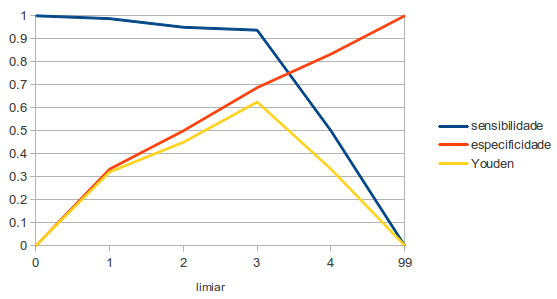
\includegraphics[scale=0.5]{img/threshold.png}
\caption{Variação dos valores de avaliação conforme o limiar de detecção}
\label{fraud:threshold}
\end{figure}

No lado esquerdo, onde o limiar é muito baixo, a sensibilidade é 1 e a especificidade, zero; enquanto no lado direito, onde o limiar é muito alto, ocorre o oposto: a sensibilidade é zero e a sensibilidade, 1. Conforme o limiar aumenta (começando do lado esquerdo e caminhando para a direita), ocorreu uma diminuição na especificidade (algumas instâncias fraudulentas começam a ser classificadas como legítimas). No entanto, há um aumento muito maior na especificidade (instâncias legítimas começam a ser classificadas corretamente). É possível ver como o índice de Youden mostra a real proporção entre esses dois valores. Uma forma mais sucinta para apresentar esse tipo de informação é através de um gráfico dos valores de sensibilidade e 1 - especificidade, que é denominado ROC (característica operativa do receptor, \emph{receiver operating characteristic}), conforme mostrado na figura \ref{fraud:roc}.

\begin{figure}[h!]
\centering
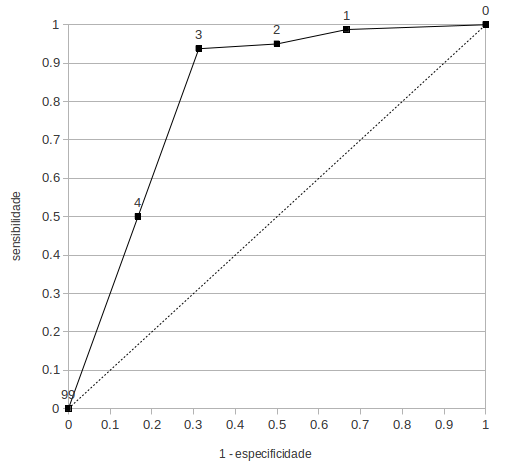
\includegraphics[scale=0.5]{img/roc.png}
\caption{Gráfico da curva ROC dos valores de exemplo}
\label{fraud:roc}
\end{figure}

No gráfico é visualmente aparente que o valor 3 como limiar de classificação oferece o melhor balanceamento entre sensibilidade e especificidade. Também é possível perceber como as alterações no limiar influenciam a distribuição desses dois valores. Um teste perfeito, que classificasse todas as instâncias corretamente, teria ambos os valores iguais a 1, tendo portanto um ponto no canto superior esquerdo do gráfico. Os pontos mais próximos dessa localização são aqueles que melhor classificam as instâncias.

Caso as instâncias fossem classificadas aleatoriamente, tendo chances iguais de serem classificadas tanto positivas quanto negativas, a sensibilidade e a especificidade seria ambas 0.5, e o teste não teria qualquer valor. Essa situação é representada pela linha diagonal entre os pontos (0, 1) e (1, 0). Essa linha é outro indicador visual útil: testes abaixo dela (na direção do canto inferior direito) têm muito pouco valor; testes próximos dela têm valor mediano; e testes acima (na direção do canto superior esquerdo) têm grande valor.

Uma das maneiras de quantificar a (dar um valor à) validade de um atributo como variável de diagnóstico é através do cálculo dá área sob a curva ROC (denominada AUROC, \emph{area under the ROC curve}). O teste ideal citado acima teria área igual a 1, enquanto testes completamente aleatórios teriam área 0.5. Testes reais normalmente situam-se entre esses dois valores, com valores mais próximos de 1 representando testes mais precisos.

Essa área pode ser calculada através da soma das áreas dos trapézios: a área sob a curva entre os pontos (0.5, 0.1667) e (0.9375, 0.3125) é igual a (0.9375 - 0.5) x (0.3125 + 0.1667)/2 = 0.1048. Aplicando essa regra aos outros pontos da curva, obtêm-se uma área total de 0.8161, ou seja, uma instância fraudulenta tem 81.61\% de ter um número de ocorrências de inadimplência maior do que uma instância legítima.

\subsection{Análise de resultados}

Uma vez que possa ser quantificada, a capacidade de diagnóstico de uma variávei pode ser comparada com outras, simplesmente comparando-se as suas curvas ROC e as áreas sob essas curvas. Variáveis com uma maior área sob a curva geram diagnósticos mais confiáveis. O formato da curva também pode servir como instrumento de análise: uma variável pode ter comportamentos preferíveis caso as condições de teste sejam diferenciadas, ou para filtrar casos específicos. Por exemplo, uma variável que, para valores muito baixos de sensibilidade, apresenta uma alta taxa de especificidade pode ser usada quando quer-se favorecer a especificidade.

A área sob a curva ROC é um método útil para a medição da precisão de diagnósticos, além da comparação de performance entre diferentes testes. No entanto, ela não deve ser tomada como verdade absoluta. A sensibilidde e a especificidade podem manter-se fixas em um ambiente de testes, mas podem variar conforme as características da populaçõ analisada.

Uma consideração importante quando analisa-se o desempenho de dois ou mais sistemas é que muito difícil (ou até mesmo impossível) excluir-se todos os fatores externos, resultando em uma análise completamente imparcial. Nesse caso específico, o resultado dos testes em cada algoritmo é fortemente influenciado pelas características dos dados na base de dados, embora os métodos de análise dos resultados procuram minimizar essa influência.

\iffalse

Uma alternativa é atribuir uma pontuação a cada instância de acordo com uma razão entre a similaridade com casos conhecidos de fraude e a dissimilaridade com casos legais.

\citet{Aral2011} utilizam o número de falsos positivos, falsos negativos e verdadeiros positivos como medida de performance do seu sistema.

\section{Trabalhos relacionados}

Colocar na introdução

O sistema detecção de fraude no comércio eletrônico apresentado em \citet{Huang2010} é um exemplo de sistema que combina dois dois processos de diferentes granularidades que interagem entre si.

\citet{Aral2011} apresentam um sistema de detecção de fraude em prescrições médicas que calcula um fator de risco associado a cada prescrição. Matrizes de incidências são geradas através de uma medida de distância entre valores cruzados (\emph{cross-features}) de uma base de conhecimento. Dessas matrizes são geradas matrizes de riscos, e cada instância da base de dados cujo risco for maior que um limiar é relatada como uma possível fraude. Os autores indicam que o raciocínio por trás desse modelo é de que os padrões no comportamento fraudulento são \emph{outliers} quando considerados no contexto do \emph{dataset} como um todo. Os limiares são configuráveis, permitindo ao usuário um controle sobre o número de falsos positivos gerados.

\fi

\chapter{Proposta}

Conforme apresentado nos capítulos anteriores, a modelagem de um sistema de detecção de fraude com a utilização de técnicas inspiradas no sistema imunológico natural busca trazer diversas vantagens tanto no processo de planejamento quanto na sua arquitetura final. Esse trabalho busca identificar exatamente \emph{quanto} esses modelos podem aperfeiçoar os métodos existentes. O método utilizado é a comparação dos resultados da classificação de algoritmos tradicionais e Sistemas Imunológicos Artificiais sobre um mesmo conjunto de dados. Esta seção apresenta os elementos principais para o desenvolvimento da proposta.

\section{Descrição geral}

Os principais elementos no desenvolvimento do trabalho são: os conjuntos de dados utilizados na execução dos testes, os algoritmos que serão testados nesses dados e os métodos de avaliação dos resultados.

\subsection{Descrição dos dados}

Para os testes serão utilizados dois conjuntos de dados contendo informações de contas de cartões de crédito. Esses dados estão disponíveis publicamente e fazem parte de um projeto chamado StatLog \cite{Michie1994}. Esse projeto foi concebido para testar diversos métodos de classificação em problemas grandes e comercialmente relevantes, comparando os seus resultados e determinando o quanto eles atendiam as necessidades da indústria. Conforme a sua própria descrição, os objetivos do projeto eram três:

\begin{enumerate}[a)]
    \item Possibilitar medidas críticas de desempenho para procedimentos de classificação disponíveis,
    \item Indicar a natureza e escopo dos desenvolvimentos futuros necessários para que os métodos atendam as necessidades e expectativas dos usuários e
    \item Indicar as direções mais promissoras de desenvolvimento para abordagens comercialmente imaturas.
\end{enumerate}

Os conjuntos de dados são denominados German Credit (Cr.Ger) e Australian Credit (Cr.Aust). Ambos contém informações sobre contas de crédito, conforme apresentado nas próximas seções.

\subsubsection{Cr.Ger}

Esse conjunto de dados foi cedido pelo professor Hans Hoffman, da Universidade de Hamburgo. Os atributos e valores que esses atributos podem assumir são descritos na listagem \ref{lst:ge_dataset} (traduzido do original)\footnote{Na descrição dos atributos, DM significa \emph{deutsche mark} (marco alemão), a moeda corrente na Alemanha na época da coleta dos dados. Para efeito de comparação, o Banco Central Europeu estipulou a conversão irrevogável do marco alemão, a partir de 1º de janeiro de 1999, em DM 1.95583 = \euro 1 (http://www.ecb.int/press/pr/date/1998/html/pr981231$\textunderscore$2.en.html).}.

\vspace{1cm}
\begin{lstlisting}[caption=Atributos do conjunto de dados alemão,label=lst:ge_dataset]
    Atributo 1: (qualitativo)
    Situação da conta corrente existente
    A11 : ... < 0 DM
    A12 : 0 <= ... < 200 DM
    A13 : ... >= 200 DM
    A14 : sem conta corrente

    Atributo 2: (numérico)
    Duração em meses

    Atributo 3: (qualitativo)
    Histórico de crédito
    A30 : nenhum crédito retirado / todos os créditos pagos apropriadamente
    A31 : todos os créditos nesse banco pagos apropriadamente
    A32 : créditos existentes pagos apropriadamente até agora
    A33 : atraso no pagamento no passado
    A34 : conta crítica / outros créditos existentes (não nesse banco)

    Atributo 4: (qualitativo)
    Propósito
    A40 : carro (novo)
    A41 : carro (usado)
    A42 : móveis/equipamento
    A43 : rádio/televisão
    A44 : eletrodomésico
    A45 : reparos
    A46 : educação
    A47 : (férias - não existe no conjunto de dados)
    A48 : reciclagem profissional
    A49 : negócios
    A410 : outros

    Atributo 5: (numérico)
    Quantidade de crédito

    Atributo 6: (qualitativo)
    Poupança
    A61 : ... < 100 DM
    A62 : 100 <= ... < 500 DM
    A63 : 500 <= ... < 1000 DM
    A64 : .. >= 1000 DM
    A65 : desconhecido / sem poupança

    Atributo 7: (qualitativo)
    Emprego atual desde
    A71 : desempregado
    A72 : ... < 1 ano
    A73 : 1 <= ... < 4 anos
    A74 : 4 <= ... < 7 anos
    A75 : .. >= 7 anos

    Atributo 8: (numérico)
    Taxa de parcelamento em porcentagem do rendimento disponível

    Atributo 9: (qualitativo)
    Estado civil e sexo
    A91 : masculino : divorciado/separado
    A92 : feminino : divorciada/separada/casada
    A93 : masculino : solteiro
    A94 : masculino : casado/viúvo
    A95 : feminino : solteira

    Atributo 10: (qualitativo)
    Outros devedores / fiadores
    A101 : nenhum
    A102 : devedor solidário
    A103 : fiador

    Atributo 11: (numérico)
    Residência atual desde

    Atributo 12: (qualitativo)
    Propriedade
    A121 : imóvel
    A122 : se não A121 : financiamento / seguro de vida
    A123 : se não A121/A122 : carro ou outro, não incluso no atributo 6
    A124 : desconhecido / sem propriedade

    Atributo 13: (numérico)
    Idade em anos

    Atributo 14: (qualitativo)
    Outros planos de parcelamento
    A141 : banco
    A142 : lojas
    A143 : nenhum

    Atributo 15: (qualitativo)
    Residência
    A151 : alugada
    A152 : própria
    A153 : gratuita

    Atributo 16: (numérico)
    Número de créditos existentes nesse banco

    Atributo 17: (qualitativo)
    Emprego
    A171 : desempregado / sem proficiência / não-doméstico
    A172 : sem proficiência / doméstico
    A173 : proficiente / funcionário público
    A174 : administrador / auto-empregado /
           empregado altamente qualificado / oficial

    Atributo 18: (numérico)
    Número de dependentes

    Atributo 19: (qualitativo)
    Telefone
    A191 : nenhum
    A192 : sim, registrado sob o nom do consumidor

    Atributo 20: (qualitativo)
    Trabalhador estrangeiro
    A201 : sim
    A202 : não
\end{lstlisting}

\subsubsection{Cr.Aust}

Os atributos do conjunto de dados australiano são descritos na listagem \ref{lst:prop_au_dataset} (traduzido do original). Uma grande desvantagem, muito comum nesse tipo de conjunto de dados (seção \ref{fraud:data}), é a de o nome dos campos ter sido alterado, perdendo o significado original. Para garantir a privacidade das informações contidas no conjunto de dados, provavelmente por questões competitivas, a empresa que cedeu os dados utilizou um processo de anonimização, garantindo que as informações confidenciais não possam ser recuperadas.

Os dados ainda podem ser utilizados para a validação de sistemas de detecção, mas não é possível saber de que forma o sistema chegou ao diagnóstico, tornando o resultado bem menos útil.

\vspace{1cm}
\begin{lstlisting}[caption=Atributos do conjunto de dados Cr.Aust, label=lst:prop_au_dataset]
A1: b, a
A2: contínuo
A3: contínuo
A4: u, y, l, t
A5: g, p, gg
A6: c, d, cc, i, j, k, m, r, q, w, x, e, aa, ff
A7: v, h, bb, j, n, z, dd, ff, o
A8: contínuo
A9: t, f
A10: t, f
A11: contínuo
A12: t, f
A13: g, p, s
A14: contínuo
A15: contínuo
A16: +,- (atributo de classe)
\end{lstlisting}

\subsection{Algoritmos}

Os algoritmos que serão utilizados para a comparação são um pacote de algoritmos desenvolvido por Jason Brownlee \cite{Brownlee2011w}, na versão mais atual (1.8, maio de 2011). Esse pacote foi especialmente desenvolvido para a plataforma de aprendizagem de máquina Weka (descrita na seção \ref{sec:prop_weka}) e são disponibilizados através de uma licença aberta (GNU GPL). Nele, são implementados diversas categorias de algoritmos de Redes Neurais e Sistemas Imunológicos Artificiais:

\begin{enumerate}
    \item Redes neurais
    \begin{enumerate}[a)]
        \item \textbf{Learning Vector Quantization (LVQ)}: similar às redes neurais, que utiliza aprendizagem supervisionada, baseada em protótipos, para classificação de dados. É similar ao algoritmo de k-vizinhos mais próximos e um precursor do próximo algoritmo.
        \item \textbf{Self-Organizing Map (SOM)}: algoritmo de redes neurais que utiliza aprendizagem não-supervisionada. Mapeia os valores da base de dados produzindo um mapa: um espaço de duas dimensões, uma representação discreta dos dados de entrada.
        \item \textbf{Feed-Forward Artificial Neural Network (FF-ANN)}: tipo de algoritmo de redes neurais onde o sinal é propagado na direção entrada-saída, sem conexões de \emph{feedback}.
    \end{enumerate}
    \item Sistemas Imunológicos Artificiais
    \begin{enumerate}[a)]
        \item \textbf{Artificial Immune Recognition System (AIRS)}: algoritmo imunológico supervisionado descrito na seção \ref{sec:prop_airs}.
        \item \textbf{Clonal Selection Algorithm (CLONALG)}: um dos principais algoritmos imunológicos, o algoritmo da seleção clonal, descrito na seção \ref{sec:ais_clonalg}.
        \item \textbf{Immunos-81}: algoritmo imunológico descrito na seção \ref{sec:prop_immunos}.
    \end{enumerate}
\end{enumerate}

Desses, os algoritmos de Sistemas Imunológicos Artificiais (2) serão utilizados para comparação com os métodos tradicionais. O algoritmo da seleção clonal (CLONALG) foi descrito na seção \ref{sec:ais_clonalg}. Os outros dois são descritos nas próximas seções. A figura \ref{fig:prop_wekaais} mostra esses algoritmos conforme apresentados na interface do WEKA.

\begin{figure}[h!]
    \centering
    \caption{Algoritmos no WEKA}
    \label{fig:prop_wekaais}
    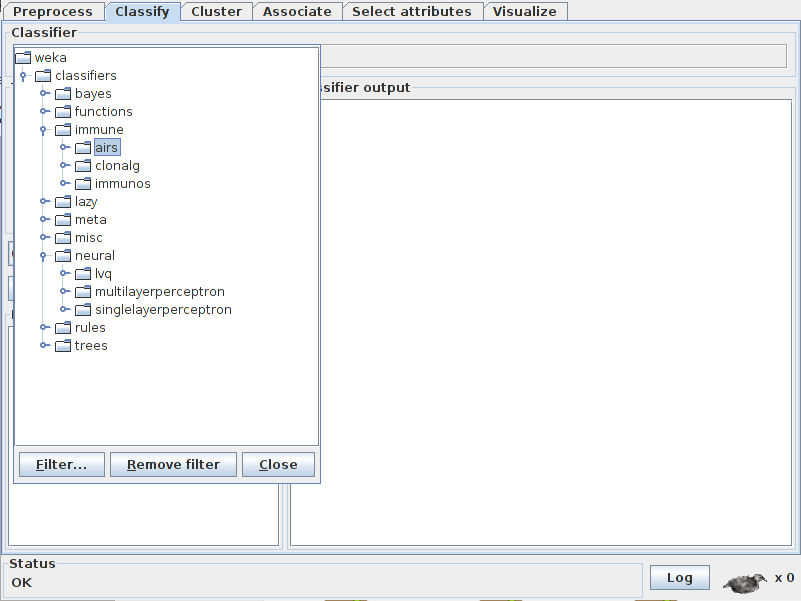
\includegraphics[width=0.75\textwidth]{img/weka_ais.png}
\end{figure}

\subsubsection{AIRS}
\label{sec:prop_airs}

Esse algoritmo foi criado por Andrew Watkins \cite{Andrew2003} e tinha como objetivo implementar um Sistema Imunológico Artificial que utilizasse aprendizagem supervisionada. Na época de seu desenvolvimento, a área de algoritmos imunológicos supervisionados não havia sido explorada, apesar da pesquisa intensa na área de algoritmos imunológicos não-supervisionados \footnote{De acordo com o autor, o único outro algoritmo imunológico supervisionado era o Immunos, apresentado na próxima seção.}

Por esse motivo, esse foi o primeiro algoritmo supervisionado a implementar a maior parte das técnicas inspiradas nos sistemas imunológicos, como: modelagem dos dados como antígenos e anticorpos, expansão clonal dos linfócitos, mutação e maturação de afinidade e memória imunológica.

Na definição desse algoritmo também foi aplicado o formalismo do espaço de formas. Conforme apresentado na seção \ref{sec:ais_shape}, esse é um formalismo bastante apropriado para a modelagem de Sistemas Imunológicos Artificiais, devido a forte semelhança entre o espaço de formas e as diferentes formas que os receptores dos linfócitos no sistema imunológico apresentam. Os antígenos identificados por esses receptores formam a região de reconhecimento ao redor de cada ponto no espaço de formas. Em um algoritmo de aprendizagem, isso representa a correspondência entre as instâncias de treinamento (antígenos) e as possíveis soluções (células B).

\subsubsection{Immunos}
\label{sec:prop_immunos}

Esse algoritmo foi apresentado por Jerome Carter \cite{Carter2000}. O algoritmo Imunnos foi desenvolvido em oposição aos algoritmos que tentavam simular fielmente o comportamento do sistema imunológico. Segundo o autor, do ponto de vista da computação, construir um sistema que utilize equações cuidadosamente derivadas dos estudos teóricos a imunologia seria um feito notável, mas não ideal. Os elementos do sistema imunológico foram reduzidos ao nível mais fundamental para que fossem introduzidos no sistema.

O principal elemento na modelagem do algoritmo foi a utilização de pequenas e simples unidades de processamento conectadas em paralelo, como pode ser observado nos nodos das redes neurais e linfócitos do sistema imunológico. As principais metas da modelagem eram:

\begin{enumerate}[a)]
    \vspace{2mm}
    \itemsep1pt
    \item Representação interna simples de ser entendida,
    \item Capacidade de generalização sobre os dados de entrada,
    \item Tempos de treinamento previsíveis,
    \item Aprendizagem \emph{online},
    \item Potencial para atuar como memória associativa,
    \item Suporte a atributos contínuos e qualitativos,
    \item Capacidade de aprendizagem e recuperação de um grande número de padrões,
    \item Aprendizagem baseada em experiência e
    \item Aprendizagem supervisionada.
    \vspace{2mm}
\end{enumerate}

\subsection{Weka}{}
\label{sec:prop_weka}

Como plataforma de testes será utilizado o \emph{software} Weka. Weka (\emph{Waikato Environment for Knowledge Analysis}, Ambiente para Aprendizagem de Máquina de Waikato) é uma suite de aplicações de aprendizagem de máquina desenvolvida na Universidade de Waikato na Nova Zelândia. Essa ferramenta é largamente utilizada em projetos nessa área, devido a sua licença aberta (GNU GPL), que permite que seja utilizada quase sem restrições.

A figura \ref{fig:prop_weka} mostra uma captura de tela do programa em execução, mostrando a visualização de um conjunto de dados de exemplo.

\begin{figure}[h!]
    \centering
    \caption{Janela do módulo Explorer - Weka 3.6.4}
    \label{fig:prop_weka}
    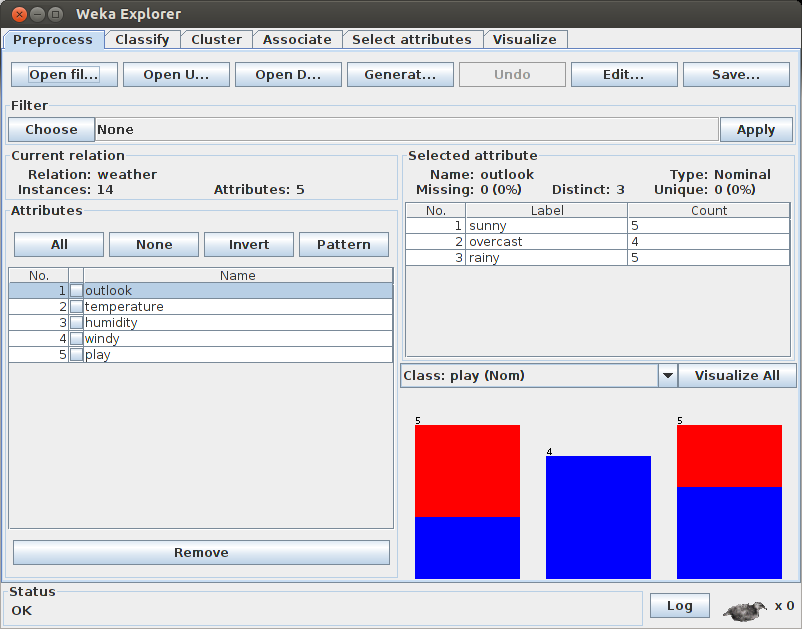
\includegraphics[width=0.75\textwidth]{img/weka.png}
\end{figure}

\iffalse arff file format \fi

A listagem \ref{lst:prop_weka_out} mostra um exemplo dos dados de saída após a execução de um teste de um dos algoritmos (LVQ) em um conjunto de dados de teste.

\vspace{1cm}
\begin{lstlisting}[caption=Exemplo de saída de uma execução do WEKA, label=lst:prop_weka_out]
    === Run information ===

    Scheme:       weka.classifiers.neural.lvq.MultipassLvq -A
    "weka.classifiers.neural.lvq.Olvq1 -M 1 -C 20 -I 1000 -L 1 -R 0.3 -S 1 -G
    false" -B "weka.classifiers.neural.lvq.Lvq3 -M 1 -C 20 -I 10000 -L 1 -R 0.05 -S
    1 -G false -W 0.3 -E 0.1"
    Relation:     weather
    Instances:    14
    Attributes:   5
                  outlook
                  temperature
                  humidity
                  windy
                  play
    Test mode:    10-fold cross-validation

    === Classifier model (full training set) ===

    -- Training Time Breakdown --
    Pass 0: 17ms
    Pass 1: 51ms
    Total Model Preparation Time: 68ms

    -- Cass Distribution --
    yes :  15 (75%)
    no :  5 (25%)



    Time taken to build model: 0.07 seconds

    === Stratified cross-validation ===
    === Summary ===

    Correctly Classified Instances           5               35.7143 %
    Incorrectly Classified Instances         9               64.2857 %
    Kappa statistic                         -0.4651
    Mean absolute error                      0.6429
    Root mean squared error                  0.8018
    Relative absolute error                135      %
    Root relative squared error            162.5137 %
    Total Number of Instances               14

    === Detailed Accuracy By Class ===

                   TP Rate   FP Rate   Precision   Recall  F-Measure   ROC Area
    Class
                     0.556     1          0.5       0.556     0.526      0.278
    yes
                     0         0.444      0         0         0          0.278
    no
    Weighted Avg.    0.357     0.802      0.321     0.357     0.338      0.278

    === Confusion Matrix ===

     a b   <-- classified as
     5 4 | a = yes
     5 0 | b = no
\end{lstlisting}

\section{Método de pesquisa}

As atividades da segunda etapa do Trabalho de Conclusão de Curso serão desenvolvidas conforme apresentadas na tabela \ref{tab:prop_cron} e serão descritas à seguir.

A etapa de coleta e preparação de dados envolverá a adaptação dos dados nos conjuntos ao formato de entrada esperado pelo WEKA, já que eles se encontram em estado bruto. O formato mais comum para utilização nesse programa são arquivos \emph{Attribute Relationship File Format} (ARFF, Formato de Arquivo de Atributo-Relação). Um arquivo nesse formato é apresentado na listagem \ref{lst:prop_arff}. Esse mesmo arquivo foi apresentado na figura \ref{fig:prop_weka}, mostrando a visualização pela interface do WEKA.

\vspace{1cm}
\begin{lstlisting}[caption=Exemplo de arquivo no formato ARFF, label=lst:prop_arff]
    @relation weather

    @attribute outlook {sunny, overcast, rainy}
    @attribute temperature real
    @attribute humidity real
    @attribute windy {TRUE, FALSE}
    @attribute play {yes, no}

    @data
    sunny,85,85,FALSE,no
    sunny,80,90,TRUE,no
    overcast,83,86,FALSE,yes
    rainy,70,96,FALSE,yes
    rainy,68,80,FALSE,yes
    rainy,65,70,TRUE,no
    overcast,64,65,TRUE,yes
    sunny,72,95,FALSE,no
    sunny,69,70,FALSE,yes
    rainy,75,80,FALSE,yes
    sunny,75,70,TRUE,yes
    overcast,72,90,TRUE,yes
    overcast,81,75,FALSE,yes
    rainy,71,91,TRUE,no
\end{lstlisting}
\vspace{1cm}

Ainda, podem ser necessários ajustes específicos nos dados para que possam servir como entrada para alguns dos algoritmos, caso estes não tenham suporte aos tipos de dados. Com os dados prontos, iniciará a fase de execução dos diferentes algoritmos sobre esses conjuntos de dados. A coleta dos resultados será feita através dos dados de saída, mostrados na listagem \ref{lst:prop_weka_out}.

Uma característica positiva da ferramenta WEKA é a possibilidade de alterar parâmetros tanto do algoritmo em si (caso eles ofereçam essa funcionalidade) quanto da execução do teste em si. Assim, pode-se executar diversos testes, variando esses parâmetros, para ao final comparar também essas configurações. A princípio, será definida apenas uma configuração, que será usada para a execução de todos os testes. No entanto, conforme for possível, poderão ser executados testes variando essa configuração, gerando comparação mais diversificadas.

De posse dos resultados dos testes de todos os algoritmos, iniciará a etapa de análise. Os resultados dos algoritmos imunológicos serão comparados com os resultados dos algoritmos tradicionais. Essa comparação envolve diversos níveis: taxas de erros e acertos (conforme apresentado na seção \ref{sec:fraud_criteria}), tempos de execução (que inclui tempo de treinamento do algoritmo e o tempo dos testes), utilização de recursos, etc. Para a visualização dos resultados, serão criados elementos visuais, como tabelas e gráficos.

Esse período também inclui a documentação do processo através da redação da monografia e a apresentação ao fim do semestre.

\begin{table}[h]
    \vspace{1cm}
    \caption{Cronograma}
    \centering
    \begin{tabular}{l >{\arraybackslash}m{4cm} >{\centering\arraybackslash}m{7cm} c}
        \multicolumn{2}{c}{Etapa} & Resultado & Data \\
        \hline
        1 & Coleta e preparação dos dados       & Arquivos no formato esperado pelo WEKA & março/2013 \\
        2 & Aplicação dos algoritmos            & Resultados da execução (taxas de acerto, métricas, tempo de execução, listagem \ref{lst:prop_weka_out} & abril/2013 \\
        3 & Comparação e análise dos resultados & Ranking de resultados & maio/2013 \\
        4 & Conclusão e contribuições           & Análise & junho/2013 \\
        5 & Redação e revisão                   & & março-julho/2013 \\
        6 & Apresentação                        & & julho/2013 \\
    \end{tabular}
    \label{tab:prop_cron}
    \vspace{1cm}
\end{table}


% Bibliografia.
\bibliography{tcc}
\bibliographystyle{abnt}

% Fim.
\end{document}

